\documentclass[10pt,a4paper]{ctexart}

% 页面设置
\usepackage[top=2.5cm, bottom=2.5cm, left=2.5cm, right=2.5cm]{geometry}

% 放宽换行要求，减少Overfull hbox警告
\sloppy

% 数学与符号
\usepackage{amsmath,amssymb,amsfonts}
\usepackage{bm}

% 图表
\usepackage{graphicx}
\usepackage{booktabs}
\usepackage{multirow}
\usepackage{subcaption}
\usepackage{array}
\usepackage{float}

% 颜色与链接
\usepackage{xcolor}
\usepackage{hyperref}
\hypersetup{
    colorlinks=true,
    linkcolor=blue,
    filecolor=magenta,
    urlcolor=cyan,
    citecolor=blue
}

% 算法
\usepackage{algorithm}
\usepackage{algorithmic}
\floatname{algorithm}{算法}
\renewcommand{\algorithmicrequire}{\textbf{输入：}}
\renewcommand{\algorithmicensure}{\textbf{输出：}}

% 代码与引用
\usepackage{listings}
\usepackage[numbers,sort&compress]{natbib}

% 其他
\usepackage{url}
\usepackage{enumitem}
\usepackage{threeparttable}

% 图片路径
\graphicspath{{figures/}}

% 标题信息
\title{\textbf{基于缺失指示器的电池健康状态预测方法对比研究：\\XJTU数据集上的深度学习模型与多缺失率实验}}
\author{作者姓名$^{1}$ \quad 通讯作者$^{2}$}
\date{$^{1}$作者单位 \\ $^{2}$通讯作者单位 \\ \texttt{email@example.com}}

\begin{document}

\maketitle

%==============================================================================
\begin{abstract}
锂离子电池健康状态（State of Health, SOH）的准确预测对于保障电动汽车和储能系统的安全可靠运行具有至关重要的意义。然而，在实际工程应用中，由于传感器故障、通信中断、数据采集异常等多种因素，电池监测数据普遍存在不同程度的缺失问题。传统的缺失数据处理方法通常将缺失视为噪声需要修复，而忽略了“哪些信息缺失”本身可能包含的有用信号，这在高缺失率场景下尤其限制了预测模型的性能上限。

本文以公开的XJTU锂离子电池数据集为研究对象，引入实现简单的缺失指示器方法（Missing Indicator Method, MIM），系统评估其在多种常用模型架构和不同缺失率条件下对SOH预测性能与鲁棒性的影响。在数据预处理阶段，我们以循环为样本单位提取16个循环级统计特征，构建循环级SOH标签；在缺失模拟阶段，通过随机方式在特征层面注入九档缺失率（Missing Rate, MR）$\{0.1, 0.2, \ldots, 0.9\}$，采用均值插补方法填补缺失值；在特征增强阶段，为每个特征构造二值缺失指示器，将“插补值与指示器拼接”作为MIM输入。我们选取了MLP、LSTM、GRU与1D-CNN四种代表性深度学习模型，在PyTorch 2.10.0深度学习框架下统一训练和评估，对比分析“仅插补”和“MIM输入”两类策略在不同缺失率下的SOH预测误差与鲁棒性差异。

实验结果表明，在缺失率$\geq 0.4$条件下，引入缺失指示器的MIM版本在四种神经网络模型中均显著降低SOH预测误差（改进率26\%--57\%）。具体而言，在MR=0.5时，1D-CNN-MIM将MAE从0.034降至0.015（改进率55.3\%），LSTM-MIM从0.022降至0.016（改进率29.0\%）。在MR=0.9的极端情况下，基线模型MAE普遍超过0.029，而MIM版本仍可维持在0.029以下，展现出显著的缺失鲁棒性。进一步的对比分析发现，不同插补方法之间的性能差异相对有限，而是否使用缺失指示器对预测性能的影响更为关键。本研究为实际电池管理系统中的数据缺失问题提供了一种简洁而有效的技术解决方案，对于提升数据驱动SOH预测方法在实际工程环境中的适用性具有重要的理论和实践价值。

\textbf{关键词：}锂离子电池；健康状态（SOH）预测；缺失数据；缺失指示器（MIM）；XJTU数据集；深度学习
\end{abstract}

%==============================================================================
\section{引言}\label{sec:intro}

\subsection{研究背景与意义}

在全球能源结构转型和交通电动化快速发展的背景下，锂离子电池作为关键储能单元，在电动汽车、电网侧储能以及分布式能源系统中得到大规模应用。准确估计与预测电池健康状态（State of Health, SOH），是保障系统运行安全、优化能量管理策略以及控制全生命周期成本的核心环节。

近年来，随着机器学习和深度学习技术的快速发展，基于数据驱动的SOH预测方法受到广泛关注\cite{luo2022review}。这类方法通过从历史运行数据中学习特征与SOH之间的复杂非线性映射关系，避免了构建和辨识复杂电化学机理模型，在适应性和可扩展性方面具有明显优势。从传统的支持向量机、随机森林等浅层模型，到多层感知机（MLP）、卷积神经网络（CNN）、循环神经网络（RNN/LSTM/GRU）等深度神经架构，各类算法在公开基准数据集上的预测精度不断提升\cite{liu2025deep}，为SOH预测的工程应用奠定了坚实基础。

然而，在实际工程场景中，一个长期被低估但十分普遍的问题是：电池管理系统（Battery Management System, BMS）采集的传感器数据往往存在不同程度的缺失。造成数据缺失的原因包括：传感器硬件故障或老化导致的测量失效，通信链路不稳定引起的数据丢包，采样策略优化导致部分通道间歇性关闭，以及整车或工况下保护机制触发导致的数据记录中断等。在大型储能电站或车队级应用场景下，由于电池数量众多、监测点密集，这一问题尤为突出。

当输入特征存在显著缺失时，传统数据驱动模型往往面临输入维度不一致、特征分布偏移和预测不确定性增加等问题；在极端情形下，模型输出可能出现失真甚至完全失效。图\ref{fig:problem_scenario}给出了BMS监测链路及对应循环级特征矩阵的示意，其中多源故障导致特征矩阵中出现随机缺失。如何在存在缺失数据的条件下维持甚至提升SOH预测性能，成为数据驱动方法走向工程落地必须正视的关键问题。

\begin{figure}[H]
    \centering
    
\includegraphics[width=0.95\textwidth]{fig1_problem_scenario.png}
    \caption{电池SOH预测中的数据缺失问题示意图。(a) BMS监测链路与潜在故障源；(b) 循环级特征矩阵与MCAR缺失模式。}
    \label{fig:problem_scenario}
\end{figure}

面对数据缺失，现有处理方式大致可以归纳为三类：删除法、插补法和基于模型的方法。删除法直接丢弃含缺失值的样本或特征，虽然实现简单，但在缺失较为普遍、且缺失模式与电池老化状态可能相关时，会导致大量信息损失并引入显著的选择偏差。插补法通过统计量（如均值、中位数）或预测模型（如回归、K近邻等）对缺失值进行估计和填补，目前在工业界应用最为广泛。然而，这类方法难以刻画由缺失引入的不确定性，且无法显式编码"哪些特征在何处缺失"这一潜在有用信息。基于模型的方法（如多重插补、基于概率图模型的缺失机制建模等）在理论上更为严谨，但往往需要复杂的分布假设，计算成本与实现难度较高，在资源受限、实时性要求较高的BMS环境中直接部署存在困难。

上述传统方法有一个共同假设：缺失是应当被"修复"的噪声，因而核心目标是"补全"数据本身，而较少关注"缺失模式"本身蕴含的信息。在许多实际场景中，这一假设并不充分。电池在老化过程中，某些传感器通道在高温、高负载工况下更容易出现异常或失效，使得缺失模式与SOH之间可能存在相关性。此时，缺失模式本身可以视作关于老化状态的间接观测量，具有潜在的诊断价值。

在此背景下，本文尝试在电池SOH预测任务中引入并系统评估一种更为简单且易于工程实现的缺失数据处理策略——缺失指示器方法（Missing Indicator Method, MIM）\cite{jones1996indicator,van2023missing}。该方法在常规插补的基础上，为每个可能缺失的特征构造对应的二值指示变量，并与插补后的特征共同输入预测模型。不同于仅关注"将缺失值补齐"的传统思路，MIM方法强调显式编码"哪些值发生了缺失"，并让模型在训练过程中一并学习特征取值与缺失模式与SOH之间的联合关系。已有研究表明，在缺失模式具有信息量（informative missingness）时，MIM在医疗数据分析、推荐系统等领域能够显著提升预测性能\cite{sisk2023imputation,ehrig2025imputation}。本文将基于公开XJTU锂离子电池数据集，通过一系列控制良好的实验，验证MIM方法在电池SOH预测任务中的有效性，并为工程实践中处理缺失数据提供定量参考。

\subsection{研究现状与不足}

在电池SOH预测领域，现有大部分研究工作是在假设数据基本完整的前提下展开的，对缺失数据问题的系统性关注仍然有限\cite{shao2025soh}。早期研究主要聚焦于在标准工况和完整数据条件下的特征工程与模型构建，例如基于完整放电曲线和完整循环数据提取容量、内阻、电压平台等特征，并采用机器学习或深度学习模型进行回归预测。典型的电信号特征建模方法包括独立成分分析（Independent Component Analysis, ICA）、差分电压分析（Differential Voltage Analysis, DVA）等，用于从电压、电流曲线中提取表征老化程度的关键特征\cite{deng2025novel}。这些方法在数据完整时能够取得较高的预测精度，但对数据完整性的依赖较强，难以直接迁移到存在广泛缺失的实际工况场景。

在缺失数据处理方面，现有研究主要集中于插补方法的改进。一类工作利用电池老化轨迹的相似性，采用K近邻等方法基于相似电池或相似循环的完整数据对缺失值进行估计；另一类工作则借助生成对抗网络（GAN）、变分自编码器（VAE）等深度生成模型，在特征空间中为缺失点合成"合理"的填充值。这些方法通常能够在一定程度上提升插补精度，但研究重心仍然围绕"更准确地补齐缺失值"。在处理流程上，缺失值一旦被填补，其"曾经缺失"的事实往往不再被显式利用。

从统计学与机器学习的视角来看，这种"仅补值、不显式建模缺失模式"的处理方式在缺失机制为完全随机缺失（Missing Completely at Random, MCAR）时是合理的；但在更常见的随机缺失（Missing at Random, MAR）或非随机缺失（Missing Not at Random, MNAR）条件下，缺失发生本身往往与已观测或未观测变量相关，此时缺失模式本身携带关于目标变量的额外信息。以电池老化过程为例，某些传感器在高温、高倍率工况下更易出现漂移、饱和或失效，使得高老化程度或特定工况下的样本更频繁地产生缺失记录。这种缺失模式本身与SOH之间的相关性，如果仅通过补值而不显式编码，很可能被传统插补流程"抹平"，从而丢失有价值的诊断信号。

缺失指示器方法（MIM）在统计与机器学习领域已有较长的研究历史，并在医疗数据分析、在线推荐系统等任务中得到广泛应用与验证\cite{jones1996indicator,van2023missing}。其核心思想是：在对缺失值进行适当插补的同时，为每个可能缺失的特征增加一个二值指示变量（缺失为1、观测为0），并将"插补特征+指示器向量"一并输入下游预测模型。已有理论与实证研究表明，当缺失机制与目标变量存在相关性时，引入缺失指示器可以显著改善模型对缺失机制的建模能力，从而提升预测性能\cite{sisk2023imputation,ehrig2025imputation}。

然而，在电池SOH预测这一具体领域，关于MIM方法的系统研究仍较为缺乏，主要体现在以下几个方面：

\begin{enumerate}[label=(\arabic*)]
    \item \textbf{缺乏统一的多缺失率评测框架}\\
    多数现有工作仅在单一或少数几个缺失率下进行验证，难以系统观测方法在缺失率从低到高（例如MR从0.1到0.9）变化过程中的性能演化，尤其缺乏对高缺失率（MR$\geq 0.6$）场景的系统评估。
    
    \item \textbf{缺乏跨架构对MIM的系统比较}\\
    电池SOH预测中常用的深度学习架构包括MLP、LSTM、GRU、1D-CNN等，不同架构在时间依赖建模、局部模式抽取及参数规模等方面具有各自优势，但其对MIM方法的适配性和受益程度如何，尚缺乏在统一设置下的横向比较。
    
    \item \textbf{公开对比实验的控制变量不足}\\
    现有文献中，不同工作之间的数据预处理流程、缺失模拟策略、模型超参数和训练设置差异较大，往往难以在同一基线上公平比较缺失处理策略的优劣。缺少在统一数据集、统一缺失模式和统一训练配置下的规范化对比实验，使得关于MIM实际收益的结论缺乏足够的可比性和说服力。
\end{enumerate}

综上所述，面向电池SOH预测任务，现有研究在多缺失率统一评测框架、跨架构MIM效果比较以及严格控制变量的公开对比实验等方面仍存在明显空白。填补这一空白，一方面有助于澄清MIM在有缺失数据条件下的真实收益及其适用边界，另一方面也为工程实践中BMS缺失数据处理策略的选择提供定量化依据。这也是本文工作的主要动机所在。

\subsection{研究目标与贡献}

针对上述研究现状与不足，本文以XJTU公开锂离子电池数据集为实验平台，以缺失指示器方法（MIM）为核心，构建了一套面向不同缺失率与多种神经网络架构的电池SOH预测实验框架，系统评估MIM在多缺失率条件下对预测性能与鲁棒性的影响。在统一的数据预处理、缺失模拟和训练配置下，本文试图回答以下三个核心研究问题（Research Questions, RQ）：

\begin{itemize}[leftmargin=2em]
    \item \textbf{RQ1（性能收益）：} 在XJTU电池数据集及设定的随机缺失条件下，相对于"仅插补"的基线输入策略，引入MIM在不同缺失率（MR=0.1--0.9）下能够带来多大的SOH预测性能提升？这种提升在不同缺失率区间上是否具有一致性与稳定性？
    
    \item \textbf{RQ2（架构差异）：} 对于MLP、LSTM、GRU、1D-CNN等典型神经网络架构，将MIM集成到输入表示中后，各架构从中获益的程度是否存在显著差异？是否存在对MIM更敏感或更鲁棒的"优选架构"组合？
    
    \item \textbf{RQ3（高缺失鲁棒性）：} 当缺失率进一步升高直至0.9等极端条件时，哪些"模型架构 + MIM"组合仍能够维持可接受的预测精度与稳定性？其误差与不确定性表现如何，可在何种程度上满足工程应用需求？
\end{itemize}

围绕上述研究问题，本文的主要贡献可概括为以下三个方面：

\begin{enumerate}[label=(\arabic*)]
    \item \textbf{方法论与框架构建：}\\
    提出并实现了一套面向缺失数据场景的电池SOH预测实验流程，将缺失指示器方法系统集成到MLP、LSTM、GRU和1D-CNN四类代表性深度学习架构中。实验框架支持多种缺失设定（包括随机缺失、区段缺失等）和两类可对比输入策略（仅插补 vs. 插补+指示器[MIM]），为后续相关研究提供了统一且可复现的实验基准。
    
    \item \textbf{系统实证与规律揭示：}\\
    在统一的数据预处理和训练设置下，本文通过多缺失率（MR=0.1--0.9）条件下、基于100个随机种子的控制变量大规模对比实验，系统量化了MIM在不同缺失率区域的性能收益，分析了不同网络架构结合MIM时的表现差异和种子稳定性，揭示了MIM收益与缺失率、模型结构之间的关系规律。
    
    \item \textbf{工程应用指导：}\\
    基于实验结果，本文在误差指标（如MAE、RMSE、R$^2$）与模型复杂度之间进行综合权衡，总结出面向不同缺失率区间和计算资源约束的模型选择建议，给出适合在实际BMS中部署的数据驱动SOH预测方案，为工程实践中处理缺失数据和选择合适的"模型+MIM"组合提供了可操作的指导意见。
\end{enumerate}

%==============================================================================
\section{相关工作}\label{sec:related}

\subsection{缺失数据处理方法与缺失指示器}

在实际数据分析任务中，数据缺失是一个普遍存在的挑战，其处理方式会直接影响后续模型训练和推断的性能。从统计学角度，缺失机制通常被分为三类：完全随机缺失（Missing Completely at Random, MCAR），即缺失与任何观测或未观测变量都无关；随机缺失（Missing at Random, MAR），即缺失可以由观测到的变量解释；以及非随机缺失（Missing Not at Random, MNAR），即缺失与未观测到的变量值本身有关\cite{little2002statistical}。在实际建模中，通常假设缺失机制满足MCAR或MAR条件，以便简化推断过程并获得更好的统计性质\cite{little2002statistical}。在不同缺失机制下，适宜的处理策略也不尽相同。

传统的缺失数据处理方法主要可以归纳为删除法、单一值插补法和基于模型的方法三大类。删除法包括列表删除（删除含缺失值的整行样本）和特征删除（删除含缺失值过多的特征列），这种方法在缺失率较低时简单有效，但在缺失率较高时会损失大量信息，且可能引入选择偏差。单一值插补方法包括均值插补、中位数插补、前向/后向填补以及基于回归模型的插补等，通过单一数值填充缺失位置，虽然保留了样本量，但会低估方差并扭曲变量间的关系。基于模型的方法如期望最大化（EM）算法、多重插补（Multiple Imputation）等通过建立概率模型处理缺失，理论上更为严谨，但计算复杂度高，通常需要对数据分布或缺失机制作出一定假设。

缺失指示器方法（Missing Indicator Method, MIM）提供了一种区别于传统删除与插补策略的建模思路\cite{jones1996indicator,van2023missing}。该方法的核心思想是将缺失信息显式编码为额外的二元特征，与原始特征共同输入模型，让模型在训练过程中学习如何利用缺失模式信息\cite{ipsen2022deal}。具体而言，对于每一个可能存在缺失的特征，都构造一个对应的指示器变量，当该特征值缺失时指示器为1，否则为0。这样，原始特征向量$X$就被扩展为$[X, M]$，其中$M$是指示器向量。这种表示方法的优势在于：模型不仅可以利用原始特征的值（经过插补后），还可以获知“该值是否被观测”这一额外信息。

从理论角度分析，MIM方法的有效性依赖于缺失机制与目标变量之间的相关性。当缺失是完全随机（MCAR）时，指示器不包含关于目标变量的信息，MIM可能仅带来边际改善甚至无改善；但当缺失与目标变量相关（MAR或MNAR）时，指示器成为有价值的预测信号，模型可以通过学习缺失模式来改进预测。在电池SOH预测场景中，部分传感器会随老化过程逐渐失效，或在特定工况下更易出现记录中断和数据缺失。此时，缺失模式往往与电池老化程度存在相关性（例如，老化程度较高的电池更易出现测量异常或数据丢失）。因此，缺失模式本身可视作关于SOH的间接观测量，在理论分析和工程应用上都具有潜在价值。

MIM方法在多个应用领域已有成功实践。在医疗数据分析中，由于患者检查项目的选择性，电子病历数据普遍存在结构化缺失，研究表明引入缺失指示器可以显著提升疾病预测模型的性能\cite{sisk2023imputation,ehrig2025imputation}。在深度学习领域，近年来有工作通过特征掩码或指示向量的方式，显式建模缺失模式，并将其作为网络输入的一部分\cite{ipsen2022deal,che2018recurrent}。此类方法通常需要对数据分布或缺失机制作出一定假设，以保证训练过程的可行性和收敛性。在推荐系统中，用户评分矩阵的稀疏性可视为一种特殊的数据缺失，通过建模“用户是否评过分”这一信号，协同过滤算法可以取得更好的推荐效果。

然而，以MIM为代表的显式缺失建模在电池SOH预测任务中的系统评估仍然稀缺，缺少在统一数据集与多缺失率条件下的对比结论。特别是在电池SOH预测这一具有强时序特性、多物理场耦合的复杂工程问题中，MIM方法的系统研究尚属空白，其在不同深度学习架构下的适用性和实际收益尚未得到充分验证。这构成了本文开展实证研究的核心动机之一。

\subsection{电池SOH预测的常用模型架构}

电池SOH预测作为典型的回归问题，其建模方法经历了从基于物理机理到数据驱动的演变过程\cite{liu2025deep}。早期的基于物理模型的方法通过建立电化学阻抗谱、等效电路模型等描述电池内部老化机制，具有明确的物理解释性，但模型参数众多、辨识困难，且难以适应不同化学体系和工况条件。随着机器学习技术的发展，数据驱动方法逐渐成为主流\cite{liu2025deep}，根据模型结构特点，可以大致分为前馈网络（MLP）、循环神经网络（LSTM/GRU）和一维卷积神经网络（1D-CNN）三类。

多层感知机（MLP）作为最基础的神经网络结构，通过多层非线性变换学习特征与SOH之间的复杂映射关系，具有实现简单、训练速度快的特点，适合作为基准方法\cite{bairwa2025cycle}。MLP、LSTM、GRU以及一维卷积（1D-CNN/TCN）等架构，已在统一数据集上被用于电池剩余寿命预测和容量重建等任务，并在真实系统中取得良好效果\cite{bairwa2025cycle}，表明不同架构在捕捉时序依赖和跨循环特征方面各具优势。MLP的优势是参数量相对可控、训练和推理效率高，适合在资源受限的嵌入式BMS中部署。然而，MLP通常将每个循环视为独立样本，难以捕捉循环间的时序依赖关系。

时序模型以长短期记忆网络（LSTM）和门控循环单元（GRU）为代表，专为处理序列数据而设计\cite{bairwa2025cycle}。与MLP相比，RNN类模型可以显式建模相邻循环之间容量与特征的时间依赖关系，这种时序建模能力是其在SOH预测任务中的主要优势。LSTM通过引入门控机制解决了传统RNN的梯度消失问题，能够有效捕捉长程依赖；GRU则通过简化门控结构在保持性能的同时降低了参数量和计算复杂度。在SOH预测中，通常将最近若干循环的特征序列作为输入，预测当前循环的SOH值。时序模型能够利用历史信息辅助当前预测，在容量再生、老化趋势转折等复杂情况下表现出更好的稳定性。

深度卷积模型主要采用一维卷积神经网络（1D-CNN），通过卷积核在时序维度上滑动提取局部特征模式\cite{zhang2024cnnsoh}。卷积与循环结构的组合可以充分利用局部电压/电流片段特征与跨循环依赖关系，在多特征SOH估计任务中已表现出优于单一结构的精度\cite{zhang2024cnnsoh}。与RNN的串行处理不同，CNN可以并行处理序列中的各个位置，训练效率更高；此外，卷积操作的平移不变性使其对循环编号的变化具有一定鲁棒性。在训练数据相对有限的条件下，1D-CNN常用于处理充放电曲线、增量容量曲线等波形数据，通过多层卷积提取从低层到高层的抽象特征。与LSTM/GRU相比，1D-CNN在捕捉长程依赖方面能力较弱，但在局部模式识别和计算效率方面具有优势。

值得注意的是，现有大多数SOH预测研究都假设输入数据基本完整，较少系统考虑数据缺失问题\cite{shao2025soh,deng2025novel}。少量工作开始关注电池温度等关键观测量中的数据缺失问题，但尚缺乏在统一数据集、多缺失率条件下的系统性对比\cite{shao2025soh}。不同神经网络架构对缺失数据的内在处理能力存在差异：CNN可以通过局部感受野提取特征，RNN可以捕捉时序依赖，而MLP作为全连接网络对缺失更为敏感。已有研究表明，针对缺失模式设计的编码策略可以显著提升时序模型的鲁棒性\cite{che2018recurrent}，本文采用的MIM方法，从输入表示层面显式编码缺失模式，与这类“将缺失视作可利用信号”的思路是一致的。

综上所述，现有深度学习SOH研究大多假设输入完整，对特征级随机缺失的鲁棒性考虑不足。不同架构对缺失数据的处理能力存在差异，但MIM在这类架构上的收益对比缺乏系统验证。这正是本文拟解决的核心问题之一。

\subsection{本研究定位与区别}

与现有文献相比，本研究的定位和主要区别体现在以下三个方面。首先，在研究视角上，现有工作多关注于提升SOH预测精度本身，而较少关注数据缺失这一实际工程中的普遍问题；本研究则将缺失数据处理作为核心研究内容，探索如何在存在缺失的条件下保持预测性能。其次，在方法选择上，现有缺失数据研究多聚焦于插补方法的改进，试图更准确地估计并填补缺失值；本研究则采用不同的思路，通过MIM方法将缺失信息显式编码，让模型自主学习如何利用这一信号。最后，在实验设计上，现有研究通常只在单一或少数缺失率下验证方法，而本研究覆盖了从0.1到0.9的九档缺失率，能够更全面地评估方法在不同缺失程度下的表现。

综上所述，本文首次在电池SOH预测领域，系统比较MIM方法在多种典型神经网络架构（MLP、LSTM、GRU、1D-CNN）和多种缺失率条件下的综合表现。通过在统一数据集和受控参数规模下开展大规模可重复实验，为缺失数据处理策略的选择提供了实证依据和工程指导。

%==============================================================================

\section{方法}\label{sec:method}

\subsection{数据集与样本构建}

本研究采用西安交通大学公开的XJTU锂离子电池数据集作为实验平台\cite{wang2024open,duan2025lithium}。该数据集已被用于构建统一的SOH深度学习基线框架\cite{wang2024open}，适合作为本研究的对比平台。该数据集包含了多种锂离子电池在不同充放电条件下的循环老化数据，涵盖了2C、3C、R2.5、R3、RW、Sim\_satellite等多个批次，电池化学体系包括磷酸铁锂（LFP）和三元材料（NMC）等主流类型。数据集中每个循环记录了详细的电压、电流、温度、容量等测量数据，为SOH预测研究提供了高质量的数据基础，已被广泛用于深度学习SOH基准研究\cite{wang2024pinn}。

在样本构建方面，本研究以循环为基本单位构建样本。对于每一个充放电循环，提取其对应的16维统计特征向量作为输入，以该循环测得的放电容量相对于初始容量的比值作为SOH标签。具体而言，SOH的计算公式定义为：
\begin{equation}
    \text{SOH}_t = \frac{Q_t}{Q_0} \times 100\%
\end{equation}
其中，$Q_t$表示第$t$个循环的实测放电容量（单位：Ah），$Q_0$表示电池初始额定容量。为了消除不同电池初始容量差异的影响，后续分析中均使用相对容量值（即SOH）而非绝对容量值。

在数据预处理阶段，我们主要执行以下步骤：

(1) \textbf{异常值剔除}。移除SOH $>$ 100\%或SOH $<$ 50\%的循环数据，这类异常点通常源于测量误差、测试中断或极端工况。

(2) \textbf{噪声平滑}。对电压、电流等连续特征进行异常检测与平滑处理，剔除明显的测量噪声。

(3) \textbf{序列对齐}。确保每个电池样本的循环序列连续完整，避免因中间缺失循环导致时序断裂，并对不同电池的循环序列进行尺度对齐，确保跨实验条件下特征表示具有可比性。

经过数据清洗后，数据集共保留约9,000个有效循环样本，覆盖从初始状态至SOH降至50\%左右的完整老化过程，为后续实验提供了充足的数据支持。

\subsection{特征工程与提取策略}

特征提取是数据驱动SOH预测的关键环节，高质量的特征能够有效表征电池的老化状态\cite{sun2025batteryhealth,wang2022chargingfeatures}。本研究从电压、电流和充电过程三个维度构建了16维循环级统计特征（见表\ref{tab:features}），作为后续缺失模拟与MIM输入的基础表示。

\textbf{电压特征}包括均值、标准差、偏度和峰度四个统计量，用于刻画电压分布的整体形态和离散程度。老化电池通常表现出更高的内阻和更显著的极化，因而其电压曲线形状会发生相应变化。

\textbf{充电过程特征}包括恒流阶段的充电电量与时间，以及电压斜率和电压熵。前两者直接反映电池的充电接受能力，斜率与熵则分别表征电压上升速率与信号复杂度。

\textbf{电流特征}包括均值、标准差、偏度、峰度，以及恒压阶段的充电电量和时间、电流斜率与电流熵。恒压阶段电流的衰减速率和波动特性是表征电池健康状态的重要指标。

所有特征在输入模型前都进行了Z-score标准化处理。在电池相关的机器学习任务中，Z-score标准化是常用预处理策略，可缓解不同特征量纲与量级差异带来的训练不稳定问题\cite{xue2024batteryml}。标准化参数（均值和标准差）仅在训练集上计算，然后统一应用于验证集和测试集，以确保数据划分的独立性和实验结果的可比性。

综上，所构建的16维循环级特征覆盖了电压、电流及充电过程的关键统计信息，能够在单次循环尺度上较全面地表征电池老化状态。后续缺失模拟与MIM输入均基于这一统一的特征表示展开。

\begin{table}[H]
\centering
\caption{循环级特征提取详情}
\label{tab:features}
\begin{tabular}{@{}llcp{6cm}@{}}
\toprule
\textbf{类别} & \textbf{特征名称} & \textbf{维度} & \textbf{物理意义} \\
\midrule
\multirow{4}{*}{电压统计} 
& voltage\_mean & 1 & 循环内电压采样值的算术平均，反映电池平均工作电压 \\
& voltage\_std & 1 & 电压标准差，表征电压波动程度 \\
& voltage\_skewness & 1 & 电压偏度，刻画电压分布不对称性 \\
& voltage\_kurtosis & 1 & 电压峰度，反映电压分布尾部特征 \\
\midrule
\multirow{4}{*}{充电特性} 
& CC\_Q & 1 & 恒流阶段充电电量（Ah），反映电池充电接受能力 \\
& CC\_time & 1 & 恒流阶段充电时间（s） \\
& voltage\_slope & 1 & 电压随时间变化斜率，与内阻相关 \\
& voltage\_entropy & 1 & 电压信号的香农熵，表征信号复杂性 \\
\midrule
\multirow{8}{*}{电流统计} 
& current\_mean & 1 & 循环内电流采样值的算术平均 \\
& current\_std & 1 & 电流标准差，表征电流波动程度 \\
& current\_skewness & 1 & 电流偏度 \\
& current\_kurtosis & 1 & 电流峰度 \\
& CV\_Q & 1 & 恒压阶段充电电量（Ah） \\
& CV\_time & 1 & 恒压阶段充电时间（s），老化电池通常更短 \\
& current\_slope & 1 & 恒压阶段电流衰减斜率 \\
& current\_entropy & 1 & 电流信号的香农熵 \\
\bottomrule
\end{tabular}
\end{table}

Z-score标准化公式定义为：
\begin{equation}
    z_{ij} = \frac{x_{ij} - \mu_j}{\sigma_j}
\end{equation}
其中，$x_{ij}$为第$i$个样本的第$j$个特征原始值，$\mu_j$和$\sigma_j$分别为训练集上第$j$个特征的均值和标准差。

\subsection{缺失模拟与插补策略}

为了系统评估不同缺失率条件下的模型性能，我们设计了九档缺失率$\{0.1, 0.2, \ldots, 0.9\}$的模拟实验。在缺失机制方面，本研究采用完全随机缺失（MCAR）机制，即在特征矩阵中按照给定比例随机选择位置置为缺失值，缺失位置的选择与特征值本身、循环编号、SOH标签等均无关。这种简化的缺失机制便于控制实验条件，也构成了评估方法缺失鲁棒性的基准场景。

缺失率（Missing Rate, MR）定义为特征矩阵中缺失元素占总元素数量的比例：
\begin{equation}
    \text{MR} = \frac{1}{n \times d} \sum_{i=1}^{n}\sum_{j=1}^{d} \mathbb{I}(x_{ij}\ \text{缺失})
    \label{eq:mr}
\end{equation}
其中，$n$为样本数量，$d$为特征维度（本研究中$d=16$），$\mathbb{I}(\cdot)$为指示函数，当条件成立时取值为1，否则为0。

在插补策略方面，本研究采用均值插补作为基础方法。对于每个缺失值，使用训练集上对应特征的均值进行填充：
\begin{equation}
    \hat{x}_{ij} = \begin{cases}
        x_{ij}, & \text{if } x_{ij} \text{ observed} \\
        \bar{x}_j, & \text{if } x_{ij} \text{ missing}
    \end{cases}
\end{equation}
其中，$\bar{x}_j$表示第$j$个特征在训练集所有样本上的均值。本研究选用均值插补作为基线插补策略。一方面，该方法计算成本较低、易于实现；另一方面，作为广泛使用的简单插补方案，它为评估在此基础上引入缺失指示器（MIM）所带来的增益提供了公平的对比基线。在仅采用插补的传统处理流程中，模型无法区分"原始观测值"和"插补得到的值"，插补本身可能引入偏差信息且难以被模型识别。为此，本文在均值插补的基础上引入MIM，通过显式标记被插补的位置，将缺失模式作为额外输入信号暴露给模型，以减轻插补误差对预测的影响。

\subsection{缺失指示器构造与输入表示}

缺失指示器（MIM）是本研究的核心方法，其构造过程如下。对于每一个原始特征，都对应构造一个二值缺失指示器变量，当该特征值缺失时指示器取值为1，被观测到时取值为0。数学上定义为：
\begin{equation}
    m_{ij} = 
    \begin{cases}
        0, & \text{if } x_{ij} \text{ observed} \\
        1, & \text{if } x_{ij} \text{ missing}
    \end{cases}
\end{equation}
其中，$m_{ij}=1$表示第$i$个样本的第$j$个特征缺失，$m_{ij}=0$表示该特征被观测到。

基于上述定义，我们构建了两种输入表示策略供对比实验使用。第一种是基线策略（Baseline），仅使用经过插补后的特征向量$\hat{X} \in \mathbb{R}^{n \times 16}$作为模型输入，这种表示方式与传统方法一致，模型无法获知哪些值是插补的。第二种是MIM策略，将插补后的特征向量与缺失指示器向量拼接，形成扩展的特征表示$[\hat{X} \,|\, M] \in \mathbb{R}^{n \times 32}$，其中$M$是16维的指示器向量。通过这种拼接，模型可以同时接收特征的值信息和缺失信息，理论上可以通过学习缺失模式与SOH之间的关系来提升预测性能。

算法\ref{alg:mim}给出了缺失指示器构造与输入表示生成的完整流程。

\begin{algorithm}[H]
\caption{缺失指示器构造与输入表示生成}
\label{alg:mim}
\begin{algorithmic}[1]
\REQUIRE 原始特征矩阵 $X \in \mathbb{R}^{n \times d}$，缺失率 $p \in [0, 1]$
\ENSURE 插补后特征 $\hat{X}$，缺失指示器 $M$，扩展输入表示 $[\hat{X} \,|\, M]$
\STATE 根据MCAR机制随机生成缺失掩码：$\Omega_{ij} \sim \text{Bernoulli}(1-p)$
\FOR{$i = 1$ to $n$}
    \FOR{$j = 1$ to $d$}
        \STATE 构造缺失指示器：$M_{ij} = \mathbf{1}(\Omega_{ij} = 0)$
        \IF{$\Omega_{ij} = 0$}
            \STATE 插补：$\hat{X}_{ij} = \bar{x}_j$ \quad \COMMENT{均值插补}
        \ELSE
            \STATE 保留原值：$\hat{X}_{ij} = X_{ij}$
        \ENDIF
    \ENDFOR
\ENDFOR
\STATE \textbf{return} $\hat{X}$, $M$, $[\hat{X} \,|\, M]$ \quad \COMMENT{返回扩展输入}
\end{algorithmic}
\end{algorithm}

图\ref{fig:baseline_vs_mim}直观展示了Baseline与MIM两种输入策略的对比。Baseline仅使用插补后的16维特征，而MIM将插补特征与16维缺失指示器拼接，形成32维扩展输入，使模型能够同时获知特征值和缺失信息。

\begin{figure}[H]
    \centering
    
\includegraphics[width=0.95\textwidth]{fig2_baseline_vs_mim.png}
    \caption{Baseline与MIM输入策略对比。(a) Baseline：仅使用插补后的特征$\hat{X} \in \mathbb{R}^{n \times 16}$；(b) MIM：将插补特征与缺失指示器拼接$[\hat{X} \,|\, M] \in \mathbb{R}^{n \times 32}$。}
    \label{fig:baseline_vs_mim}
\end{figure}

\subsection{模型架构与参数配置}

为了确保实验比较的公平性，我们对所有深度学习模型的参数规模进行了控制。为避免模型容量差异掩盖MIM带来的收益，本研究将四种模型的参数规模控制在约15,000–45,000的同一量级，使得比较更侧重于输入形式（Baseline vs. MIM）而非粗暴堆叠参数。这一范围的选择基于以下考量：（1）足够大的参数量以确保模型具有足够的表达能力来学习特征与SOH之间的复杂映射；（2）不至于过大以避免过拟合风险和过高的计算开销；（3）保持不同架构间参数量的可比性。当使用MIM输入时，由于输入维度从16增加到32，参数量相应增加，但这种增加是输入维度变化的必然结果。考虑到不同架构的最优配置可能存在差异，我们基于预实验的架构搜索确定了各模型的最优超参数配置。

\textbf{多层感知机（MLP）}采用四层隐藏层结构（192→96→48→24），使用ReLU激活函数，层间Dropout率为0.15。

\textbf{长短期记忆网络（LSTM）}采用双层循环结构，隐藏单元数为48，序列长度为5个连续循环，Dropout率为0.2。

\textbf{门控循环单元（GRU）}采用双层循环结构，隐藏单元数为64，序列长度为5，Dropout率为0.2。GRU相比LSTM具有更少的门控参数，在保持时序建模能力的同时计算效率更高。

\textbf{一维卷积神经网络（1D-CNN）}包含两层卷积层（通道数72→32），卷积核大小为4，时序维度采用AdaptiveAvgPool1d进行自适应池化，Dropout率为0.1。在相同参数规模约束下，1D-CNN在预测精度与模型复杂度之间取得了相对更优的折中（见图\ref{fig:model_architectures}(d)），体现出较高的性能-参数效率。

\begin{table}[H]
\centering
\caption{模型架构与参数配置（基于架构搜索确定的最优配置）}
\label{tab:model_config}
\begin{threeparttable}
\begin{tabular}{@{}llp{5cm}rr@{}}
\toprule
\textbf{模型} & \textbf{架构细节} & \textbf{关键超参数} & \textbf{Baseline} & \textbf{MIM} \\
\midrule
MLP & 输入$\rightarrow$192$\rightarrow$96$\rightarrow$48$\rightarrow$24$\rightarrow$1 & ReLU, Dropout=0.15 & 27,649 & 36,865 \\
LSTM & 2层LSTM$\rightarrow$全连接 & hidden=48, seq\_len=5, Dropout=0.2 & 31,537 & 40,753 \\
GRU & 2层GRU$\rightarrow$全连接 & hidden=64, seq\_len=5, Dropout=0.2 & 40,769 & 49,985 \\
1D-CNN & Conv1d(16$\rightarrow$72$\rightarrow$32)$\rightarrow$FC & kernel=4, Dropout=0.1 & 16,713 & 30,537 \\
\bottomrule
\end{tabular}
\begin{tablenotes}
    \item 注：参数量统计包含可训练权重和偏置。参数量范围控制在15,000-45,000之间，以平衡模型表达能力和计算效率。
\end{tablenotes}
\end{threeparttable}
\end{table}

图\ref{fig:model_architectures}展示了四种模型架构的结构对比。所有模型的参数量控制在15,000--45,000的同一量级，以确保实验比较的公平性。当使用MIM输入时，由于输入维度从16增加到32，参数量相应增加，但这种增加是输入维度变化的必然结果。

\begin{figure}[H]
    \centering
    
\includegraphics[width=0.95\textwidth]{fig3_model_architectures.png}
    \caption{四种深度学习模型架构对比。(a) MLP：四层全连接网络；(b) LSTM：双层长短期记忆网络；(c) GRU：双层门控循环单元；(d) 1D-CNN：两层卷积神经网络。}
    \label{fig:model_architectures}
\end{figure}

表\ref{tab:model_config}汇总了四种深度学习模型的详细架构配置。各模型的超参数（层数、神经元数量、Dropout率等）均基于架构搜索实验确定，以在参数量约束下达到最优性能。参数量范围控制在15,000-45,000之间，这一范围的选择基于以下考量：（1）足够大的参数量以确保模型具有足够的表达能力来学习特征与SOH之间的复杂映射；（2）不至于过大以避免过拟合风险和过高的计算开销；（3）保持不同架构间参数量的可比性。当使用MIM输入时（输入维度从16增至32），参数量相应增加，但这种增加是输入维度变化的必然结果。以MLP为例，参数量计算公式为：
\begin{equation}
    \text{Params}_{\text{MLP}}^{\text{Baseline}} = (16 \times 192 + 192) + (192 \times 96 + 96) + (96 \times 48 + 48) + (48 \times 24 + 24) + (24 \times 1 + 1) = 27,649
\end{equation}
\begin{equation}
    \text{Params}_{\text{MLP}}^{\text{MIM}} = (32 \times 192 + 192) + (192 \times 96 + 96) + (96 \times 48 + 48) + (48 \times 24 + 24) + (24 \times 1 + 1) = 36,865
\end{equation}
其中输入维度$d_{\text{in}}$在Baseline策略下为16，在MIM策略下为32（增加16维缺失指示器），括号内第二项为偏置参数。

\begin{table}[H]
\centering
\caption{训练超参数配置}
\label{tab:training_config}
\begin{tabular}{@{}lcl@{}}
\toprule
\textbf{超参数} & \textbf{配置值} & \textbf{说明} \\
\midrule
优化器 & Adam & 自适应学习率优化 \\
学习率 & $10^{-3}$ & 初始学习率 \\
Batch size & 32 & 小批量梯度下降 \\
最大轮数 & 200 & 早停前的最大训练轮数 \\
早停耐心 & 15 rounds & 验证损失不下降则停止 \\
损失函数 & MSE & 均方误差 \\
\bottomrule
\end{tabular}
\end{table}

表\ref{tab:training_config}列出了训练过程的关键超参数配置。所有深度学习模型均在PyTorch 2.10.0框架下实现，采用早停机制防止过拟合。

\subsection{训练策略与评价指标}

在数据集划分方面，我们按照电池单元而非循环样本进行划分，将不同电池的数据分别划入训练集、验证集和测试集，比例约为60\%/20\%/20\%。这种划分方式保证测试阶段评估的是"未见过的电池"，从而更客观地检验模型的跨电池泛化能力。

\begin{table}[H]
\centering
\caption{数据集划分详情}
\label{tab:data_split}
\begin{tabular}{@{}lcccp{5cm}@{}}
\toprule
\textbf{子集} & \textbf{比例} & \textbf{电池数} & \textbf{循环数} & \textbf{用途} \\
\midrule
训练集 & 60\% & $\approx$18 & $\approx$6,000 & 模型参数学习 \\
验证集 & 20\% & $\approx$6 & $\approx$2,000 & 超参数调优、早停 \\
测试集 & 20\% & $\approx$6 & $\approx$2,000 & 最终性能评估 \\
\bottomrule
\end{tabular}
\end{table}

表\ref{tab:data_split}展示了数据集划分的详细信息。按电池单元划分而非按循环划分至关重要，因为同一电池不同循环之间的容量存在强相关性，随机划分会导致信息泄露和过于乐观的性能估计。

针对带缺失指示器的MIM模型，仅在单一缺失率下训练可能不足以让模型充分学习不同缺失模式。为此，我们提出多缺失率联合训练策略：将完整训练集在缺失率$r \in \{0.0, 0.1, \ldots, 0.9\}$下分别生成10个带缺失副本，并通过算法\ref{alg:mim}构造对应的指示器与扩展输入，最终合并形成扩大10倍的增强训练集。在该增强集上训练得到统一的MIM模型，使其在训练阶段即可接触到多种典型缺失模式，从而提升对未知缺失条件的鲁棒性。验证集则固定采用中等缺失率$r=0.5$，用于代表性评估模型的泛化表现。相比之下，传统基线模型（无MIM）仅在完整数据（缺失率0.0）上训练，这是因为在没有缺失指示器的情况下，训练数据中的缺失只会带来噪声而无额外信息。

算法\ref{alg:training}描述了MIM模型的多缺失率联合训练流程。

\begin{algorithm}[H]
\caption{MIM模型多缺失率联合训练}
\label{alg:training}
\begin{algorithmic}[1]
\REQUIRE 完整训练集 $\mathcal{D}_{\text{train}} = \{X, Y\}$，缺失率集合 $\mathcal{P} = \{0.0, 0.1, \ldots, 0.9\}$
\ENSURE 训练好的MIM模型 $f_{\text{MIM}}$
\STATE 初始化：$\mathcal{D}_{\text{augmented}} \leftarrow \emptyset$
\FOR{$p \in \mathcal{P}$}
    \STATE 调用算法\ref{alg:mim}：$(\hat{X}^{(p)}, M^{(p)}, Z^{(p)}) \leftarrow \text{MIM-Construct}(X, p)$
    \STATE 合并：$\mathcal{D}_{\text{augmented}} \leftarrow \mathcal{D}_{\text{augmented}} \cup \{(Z^{(p)}, Y)\}$
\ENDFOR
\STATE \COMMENT{扩充后的训练集包含$10 \times n$个样本}
\STATE 初始化模型参数 $\theta$
\FOR{epoch $= 1$ to $E_{\max}$}
    \FOR{batch $\mathcal{B} \subset \mathcal{D}_{\text{augmented}}$}
        \STATE 前向传播：$\hat{Y} = f_{\text{MIM}}(Z; \theta)$
        \STATE 计算损失：$\mathcal{L} = \frac{1}{|\mathcal{B}|} \sum (Y - \hat{Y})^2$
        \STATE 反向传播更新$\theta$
    \ENDFOR
    \STATE 在验证集（缺失率0.5）上评估
    \STATE 早停检查
\ENDFOR
\STATE \textbf{return} $f_{\text{MIM}}$
\end{algorithmic}
\end{algorithm}

图\ref{fig:joint_training}形象地展示了算法\ref{alg:training}中多缺失率联合训练的具体过程。原始训练集按照10个缺失率分别生成副本，每个副本经过MIM构造后合并形成一个扩充10倍的训练集，最终训练出一个能够处理任意缺失率的统一MIM模型。

\begin{figure}[H]
    \centering
    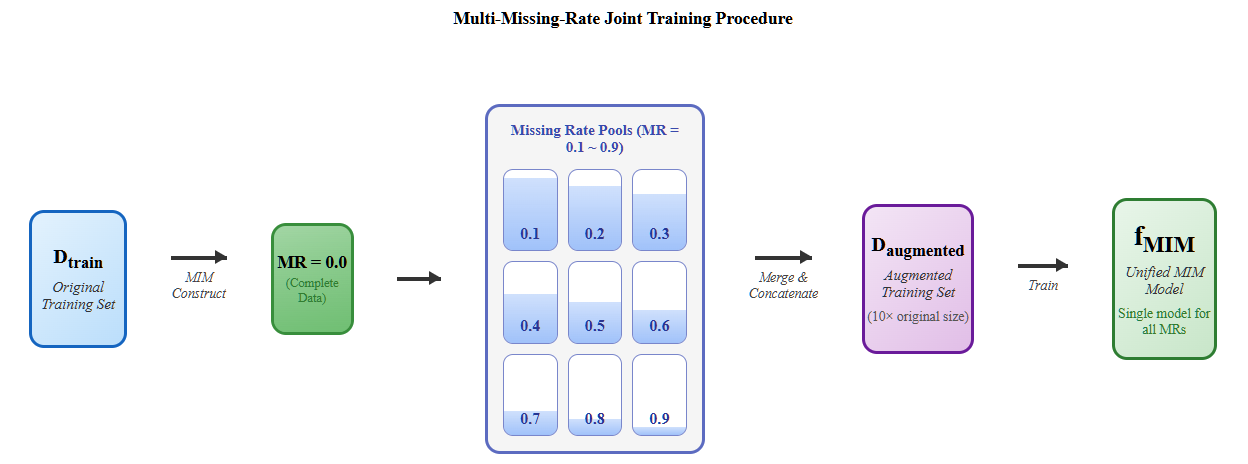
\includegraphics[width=0.95\textwidth]{fig4_joint_training.png}
    \caption{多缺失率联合训练流程。原始训练集按照缺失率$\{0.0, 0.1, \ldots, 0.9\}$生成10个副本，经MIM构造后合并为$\mathcal{D}_{\text{augmented}}$，用于训练统一的MIM模型$f_{\text{MIM}}$。}
    \label{fig:joint_training}
\end{figure}

评价指标方面，我们采用三个常用的回归评估指标\cite{jadon2022regressionloss}，其数学定义如下。MAE与RMSE是回归任务中最常用的评估指标之一，其中RMSE对大误差更加敏感，适合作为整体精度和稳定性的观测指标\cite{jadon2022regressionloss}。

平均绝对误差（Mean Absolute Error, MAE）衡量预测值与真实值之间的平均绝对偏差，对异常值相对稳健：
\begin{equation}
    \text{MAE} = \frac{1}{n} \sum_{i=1}^{n} |y_i - \hat{y}_i|
    \label{eq:mae}
\end{equation}

均方根误差（Root Mean Square Error, RMSE）对大误差有更强的惩罚，反映预测的整体精度：
\begin{equation}
    \text{RMSE} = \sqrt{\frac{1}{n} \sum_{i=1}^{n} (y_i - \hat{y}_i)^2}
    \label{eq:rmse}
\end{equation}

决定系数（Coefficient of Determination, R²）衡量模型解释数据变异的能力，值越接近1表示拟合越好：
\begin{equation}
    R^2 = 1 - \frac{\sum_{i=1}^{n} (y_i - \hat{y}_i)^2}{\sum_{i=1}^{n} (y_i - \bar{y})^2}
    \label{eq:r2}
\end{equation}
其中，$n$为样本数量，$y_i$为第$i$个样本的真实SOH值，$\hat{y}_i$为预测值，$\bar{y}$为真实值的均值。

%==============================================================================
\section{实验结果与分析}\label{sec:results}

\subsection{实验设置与整体表现}

本研究在Python 3.12与PyTorch 2.10.0环境下实现所有深度学习模型训练与评估。为了确保实验结果的统计可靠性，我们采用100个不同的随机种子（42–141）对数据划分、缺失模拟和模型训练全流程进行重复，最终报告多次重复实验的均值和标准差。

图\ref{fig:mae_curves}展示了四种模型在不同缺失率下的MAE曲线，阴影区域为基于100个随机种子的95\%置信区间。从图中可以概括出三点现象：

（1）随着缺失率的增加，所有模型的MAE均呈单调上升趋势，反映了在可用信息减少时预测任务的难度提升；

（2）在全区间内，MIM版本（实线）的MAE始终低于对应Baseline版本（虚线），表明引入缺失指示器在各缺失率下均能带来性能收益；

（3）在中高缺失率区间（MR$\geq$0.5），两种输入策略之间的性能差距明显扩大，说明MIM在数据质量较差的场景下优势更为突出。这一现象表明，在MR$\geq$0.5的条件下，MIM对抑制性能退化尤为有效，其原因可能在于缺失指示器为模型提供了区分"可靠观测"与"插补估计"的信号，使模型能够自适应地降低对插补值的依赖权重。

\begin{figure}[H]
    \centering
    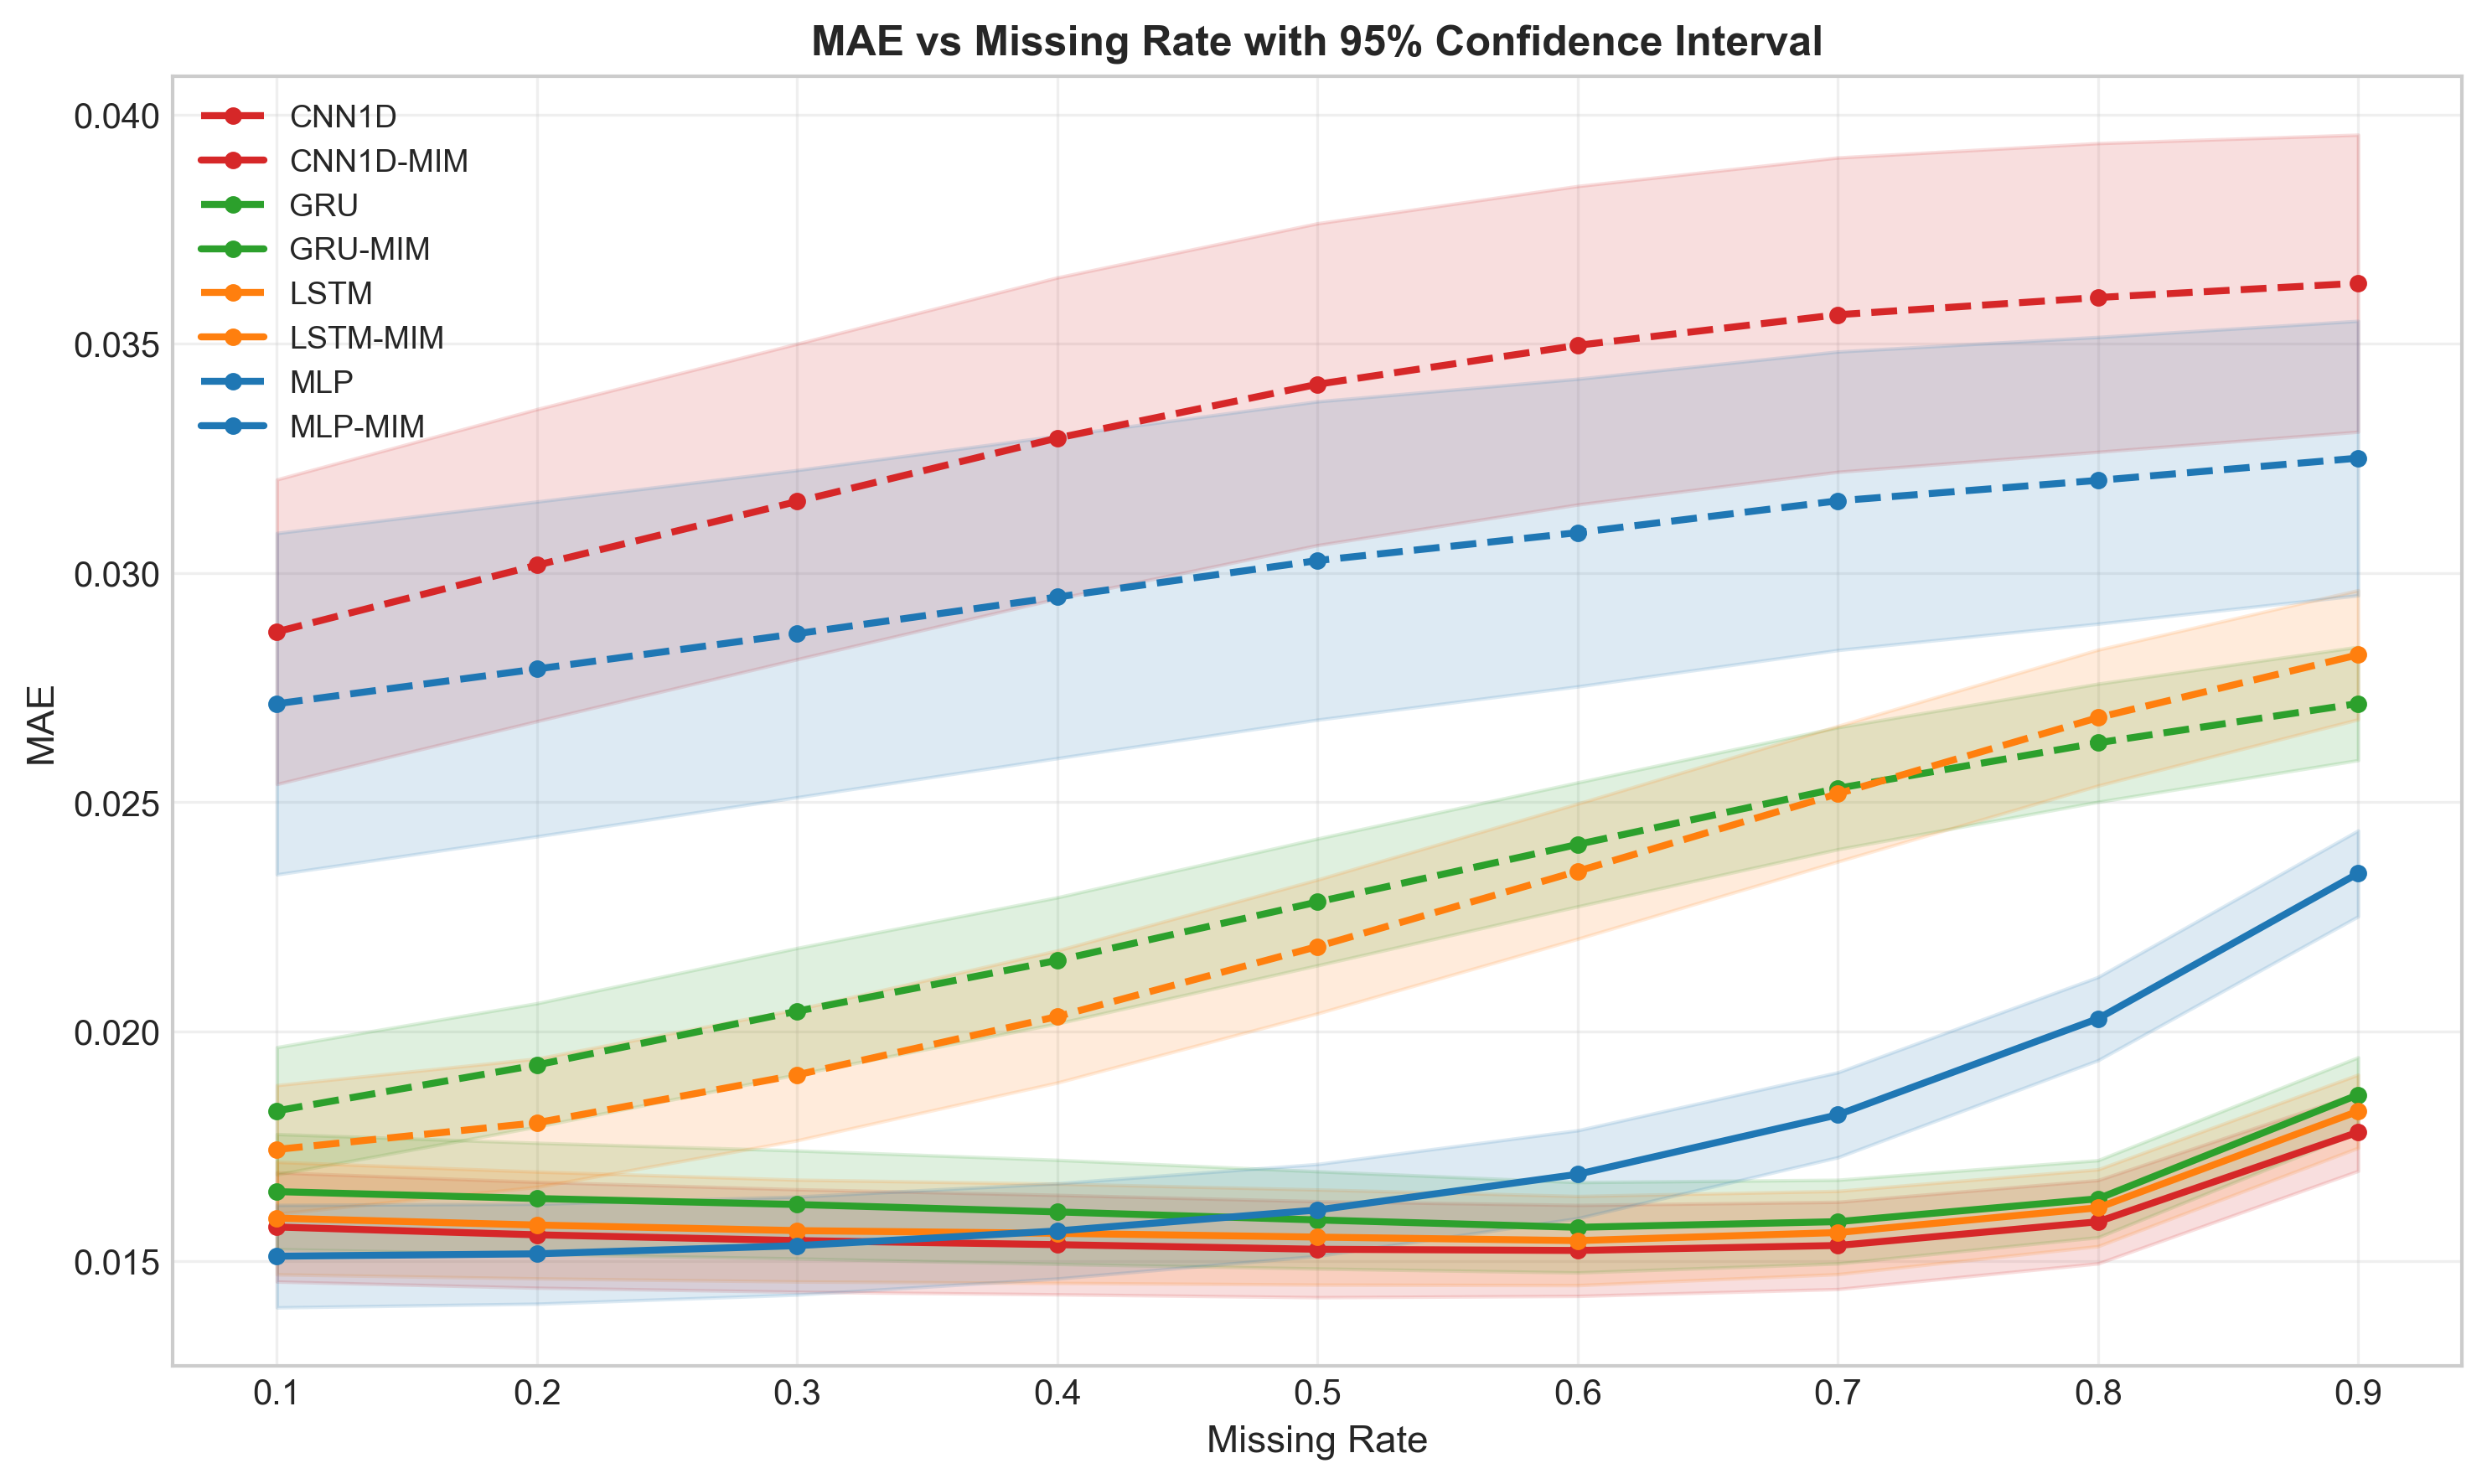
\includegraphics[width=0.95\textwidth]{mae_curves_ci.png}
    \caption{不同缺失率下各模型的MAE表现对比。实线表示使用MIM策略的模型，虚线表示仅使用插补的基线模型，阴影区域表示95\%置信区间。可以观察到MIM版本在大多数缺失率下均优于基线版本，且在高缺失率时优势更为明显。}
    \label{fig:mae_curves}
\end{figure}

表\ref{tab:full_results}给出了四个关键缺失率（0.3、0.5、0.7、0.9）下的详细数值对比。在缺失率0.5时，MLP的基线MAE为0.030$\pm$0.017，而MIM版本降至0.016$\pm$0.005，改进幅度约47\%；LSTM从0.022$\pm$0.007降至0.016$\pm$0.005，改进约29\%；GRU从0.023$\pm$0.007降至0.016$\pm$0.005，改进约30\%；1D-CNN从0.034$\pm$0.018降至0.015$\pm$0.005，改进高达55\%。所有深度学习模型在MIM输入下的MAE均低于对应的Baseline，后文的Wilcoxon符号秩检验进一步验证了这一性能差异的统计显著性。

图\ref{fig:mae_heatmap}以热力图形式展示了各模型在九种缺失率下的MAE。上半部分为Baseline，下半部分为MIM。可以看到，Baseline版本的颜色随缺失率增加明显加深，而MIM版本整体颜色更浅，且在高缺失率（MR$\geq$0.7）下仍保持较低的MAE范围。该现象与图\ref{fig:mae_curves}中的曲线趋势一致，说明MIM在高缺失率场景下对性能退化具有一定抑制作用。

\begin{figure}[H]
    \centering
    
\includegraphics[width=0.95\textwidth]{mae_heatmap.png}
    \caption{不同模型在不同缺失率下的MAE热力图（高分辨率版本，带数值标注）。行表示模型（上半部分为Baseline，下半部分为MIM），列表示缺失率。颜色越浅表示MAE越低（性能越好）。}
    \label{fig:mae_heatmap}
\end{figure}

在缺失率0.9的极端情况下，基线模型的性能出现退化，MAE相比低缺失率时有所上升，而MIM版本仍能保持相对较低的MAE（低于0.025）。这一现象表明，在MR$\geq$0.5条件下，MIM对抑制性能退化尤为有效，其原因可能在于缺失指示器为模型提供了区分"可靠观测"与"插补估计"的信号，使模型能够自适应地降低对插补值的依赖权重。

\subsection{MIM改进率分析}

为了更直观地量化MIM带来的性能提升，我们计算了改进率指标，定义为基线MAE与MIM MAE之差除以基线MAE的百分比：
\begin{equation}
    \text{Improvement}(\%) = \frac{\text{MAE}_{\text{Baseline}} - \text{MAE}_{\text{MIM}}}{\text{MAE}_{\text{Baseline}}} \times 100\%
\end{equation}
正值表示MIM优于基线，负值表示劣于基线。

图\ref{fig:improvement}展示了各模型的改进率随缺失率变化的曲线。表\ref{tab:improvement_summary}汇总了各模型在关键缺失率点的改进率数值。

\begin{table}[H]
\centering
\caption{MIM相比Baseline的MAE改进率汇总（\%）}
\label{tab:improvement_summary}
\begin{tabular}{@{}lcccccc@{}}
\toprule
\textbf{模型} & \textbf{0.1} & \textbf{0.3} & \textbf{0.5} & \textbf{0.7} & \textbf{0.9} & \textbf{平均} \\
\midrule
MLP & 44.4 & 46.5 & 46.8 & 42.4 & 27.9 & 42.5 \\
LSTM & 8.6 & 17.8 & 29.0 & 38.0 & 35.3 & 26.5 \\
GRU & 9.6 & 20.6 & 30.4 & 37.4 & 31.4 & 26.9 \\
1D-CNN & 45.2 & 51.1 & 55.3 & 57.0 & 51.0 & 52.6 \\
\bottomrule
\end{tabular}
\end{table}

从表\ref{tab:improvement_summary}可以清晰地看到，MLP、LSTM、GRU、1D-CNN四种神经网络模型的改进率在缺失率$\geq 0.4$时均为显著正值。1D-CNN的改进幅度最大，平均改进率达52.6\%，表明CNN架构对于缺失指示器信号的利用最为充分。对于LSTM和GRU，两者的改进率均随缺失率提高而逐步增加（从MR=0.3的17.8\%/20.6\%提升至MR=0.7的38.0\%/37.4\%），说明MIM对时序模型在高缺失率条件下的帮助更加显著。MLP的平均改进率为42.5\%，在较低缺失率时改进明显，但在高缺失率时改进幅度有所下降。

\begin{figure}[H]
    \centering
    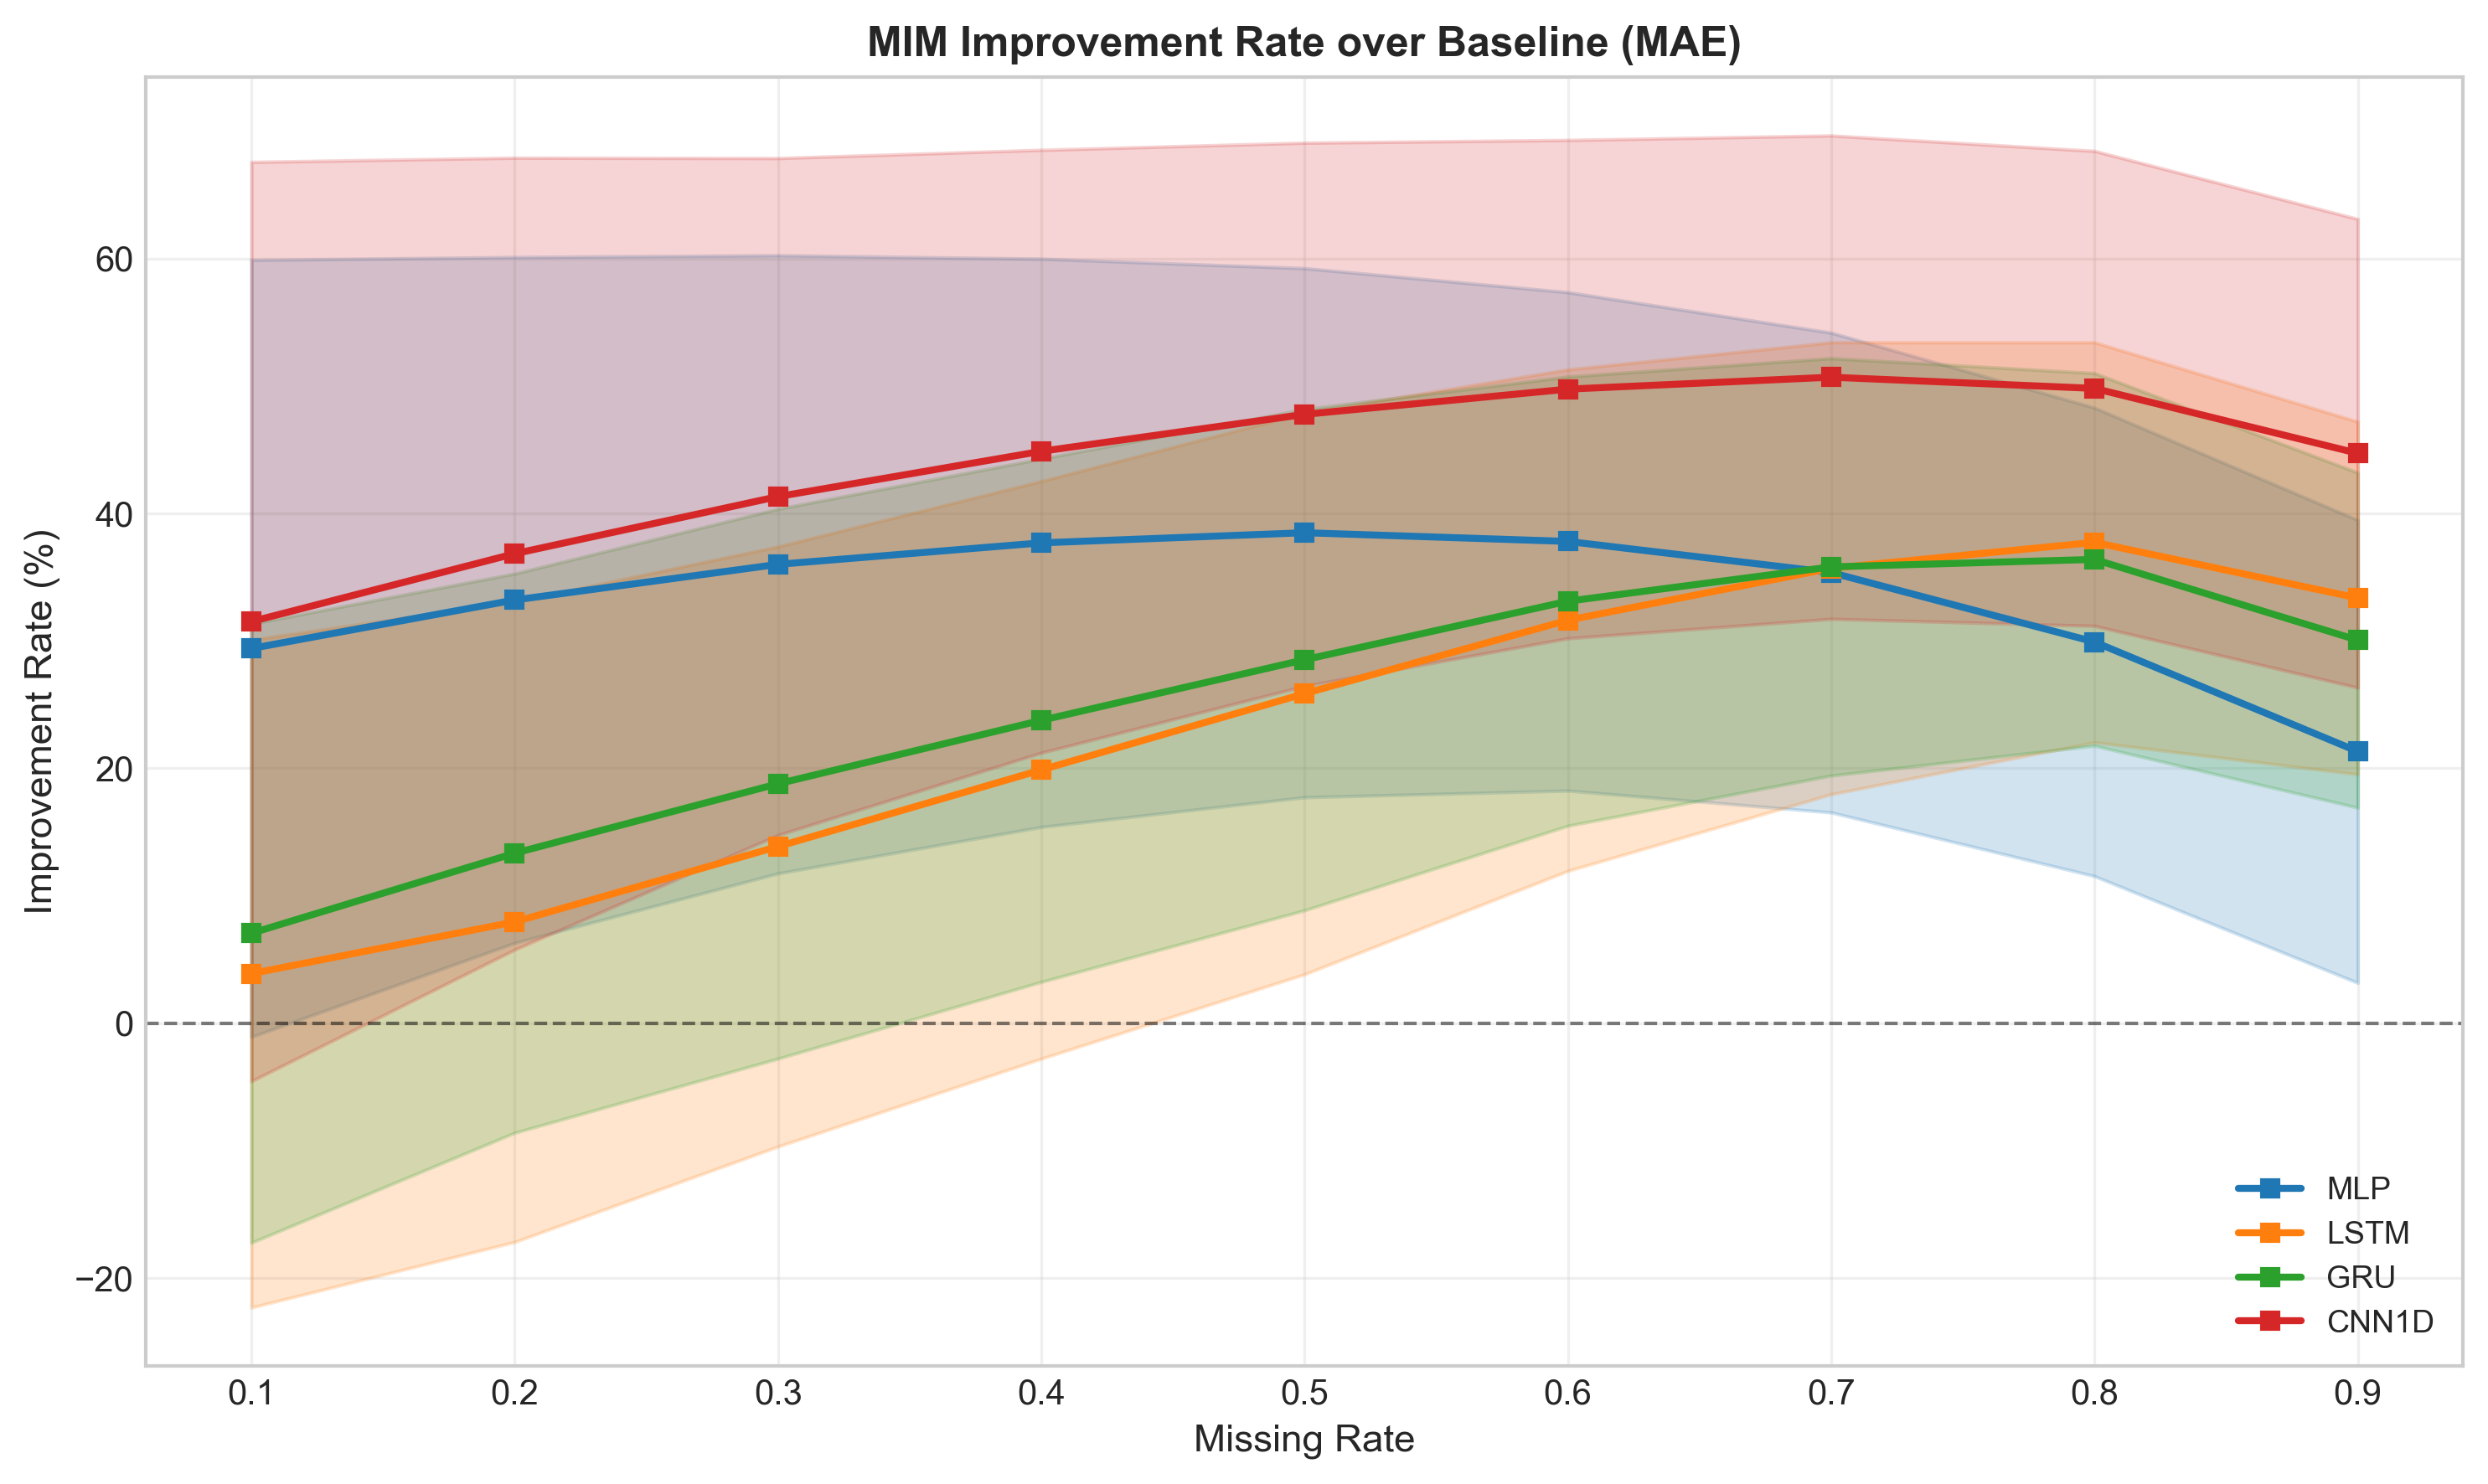
\includegraphics[width=0.95\textwidth]{mae_improvement_rate.png}
    \caption{MIM相比Baseline的MAE改进率。正值表示MIM表现优于基线，负值表示劣于基线。可以观察到神经网络模型（MLP、LSTM、GRU、CNN）在缺失率$\geq 0.4$时均有显著正向改进。}
    \label{fig:improvement}
\end{figure}

上述结果表明，MIM方法在不同神经网络架构中的收益存在差异，其中1D-CNN的平均改进率最高（52.6\%），LSTM和GRU在中高缺失率区间也获得了显著收益，而MLP在低缺失率下的相对改进更为突出。这一现象的可能解释是：CNN通过局部感受野机制能够有效利用缺失指示器区分"真实波形"与"插补伪迹"，而时序模型则可通过门控机制学习时间维度上的缺失模式依赖。

综上所述，MIM方法在四种神经网络架构中均能带来性能提升，但提升幅度和随缺失率变化的模式存在差异：1D-CNN在各缺失率区间均保持较高改进率，体现出对MIM信号的最佳利用能力；时序模型（LSTM、GRU）的改进率随缺失率提高而单调上升，说明其在高缺失率场景下的鲁棒性优势；MLP虽然在低缺失率时改进明显，但在MR$>$0.7时改进幅度有所下降，提示全连接结构对高比例缺失的适应能力相对有限。

\subsection{种子稳定性与统计显著性}

已有研究表明，随机种子的选择会显著影响深度学习模型的实验结论\cite{schader2024seed}。因此，我们在本研究中采用100个不同的随机种子，对数据划分、缺失模拟和模型训练全流程进行重复，以系统评估MIM与Baseline在多种缺失率下的稳定性差异。

对于$K=100$个随机种子，设第$k$个种子下的MAE为$e_k$，则样本均值和样本标准差定义为：
\begin{equation}
    \bar{e} = \frac{1}{K}\sum_{k=1}^{K} e_k, \quad
    s = \sqrt{\frac{1}{K-1}\sum_{k=1}^{K} (e_k-\bar{e})^2}
    \label{eq:stats}
\end{equation}
95\%置信区间为：
\begin{equation}
    \text{CI}_{95\%} = \bar{e} \pm t_{0.975, K-1}\cdot \frac{s}{\sqrt{K}}
    \label{eq:ci}
\end{equation}
图\ref{fig:seed_stability}展示了各模型在100个随机种子下的MAE曲线。灰色细线对应单个种子的结果，彩色实线和虚线分别表示MIM与Baseline在不同缺失率下的跨种子平均MAE。

\begin{figure}[H]
    \centering
    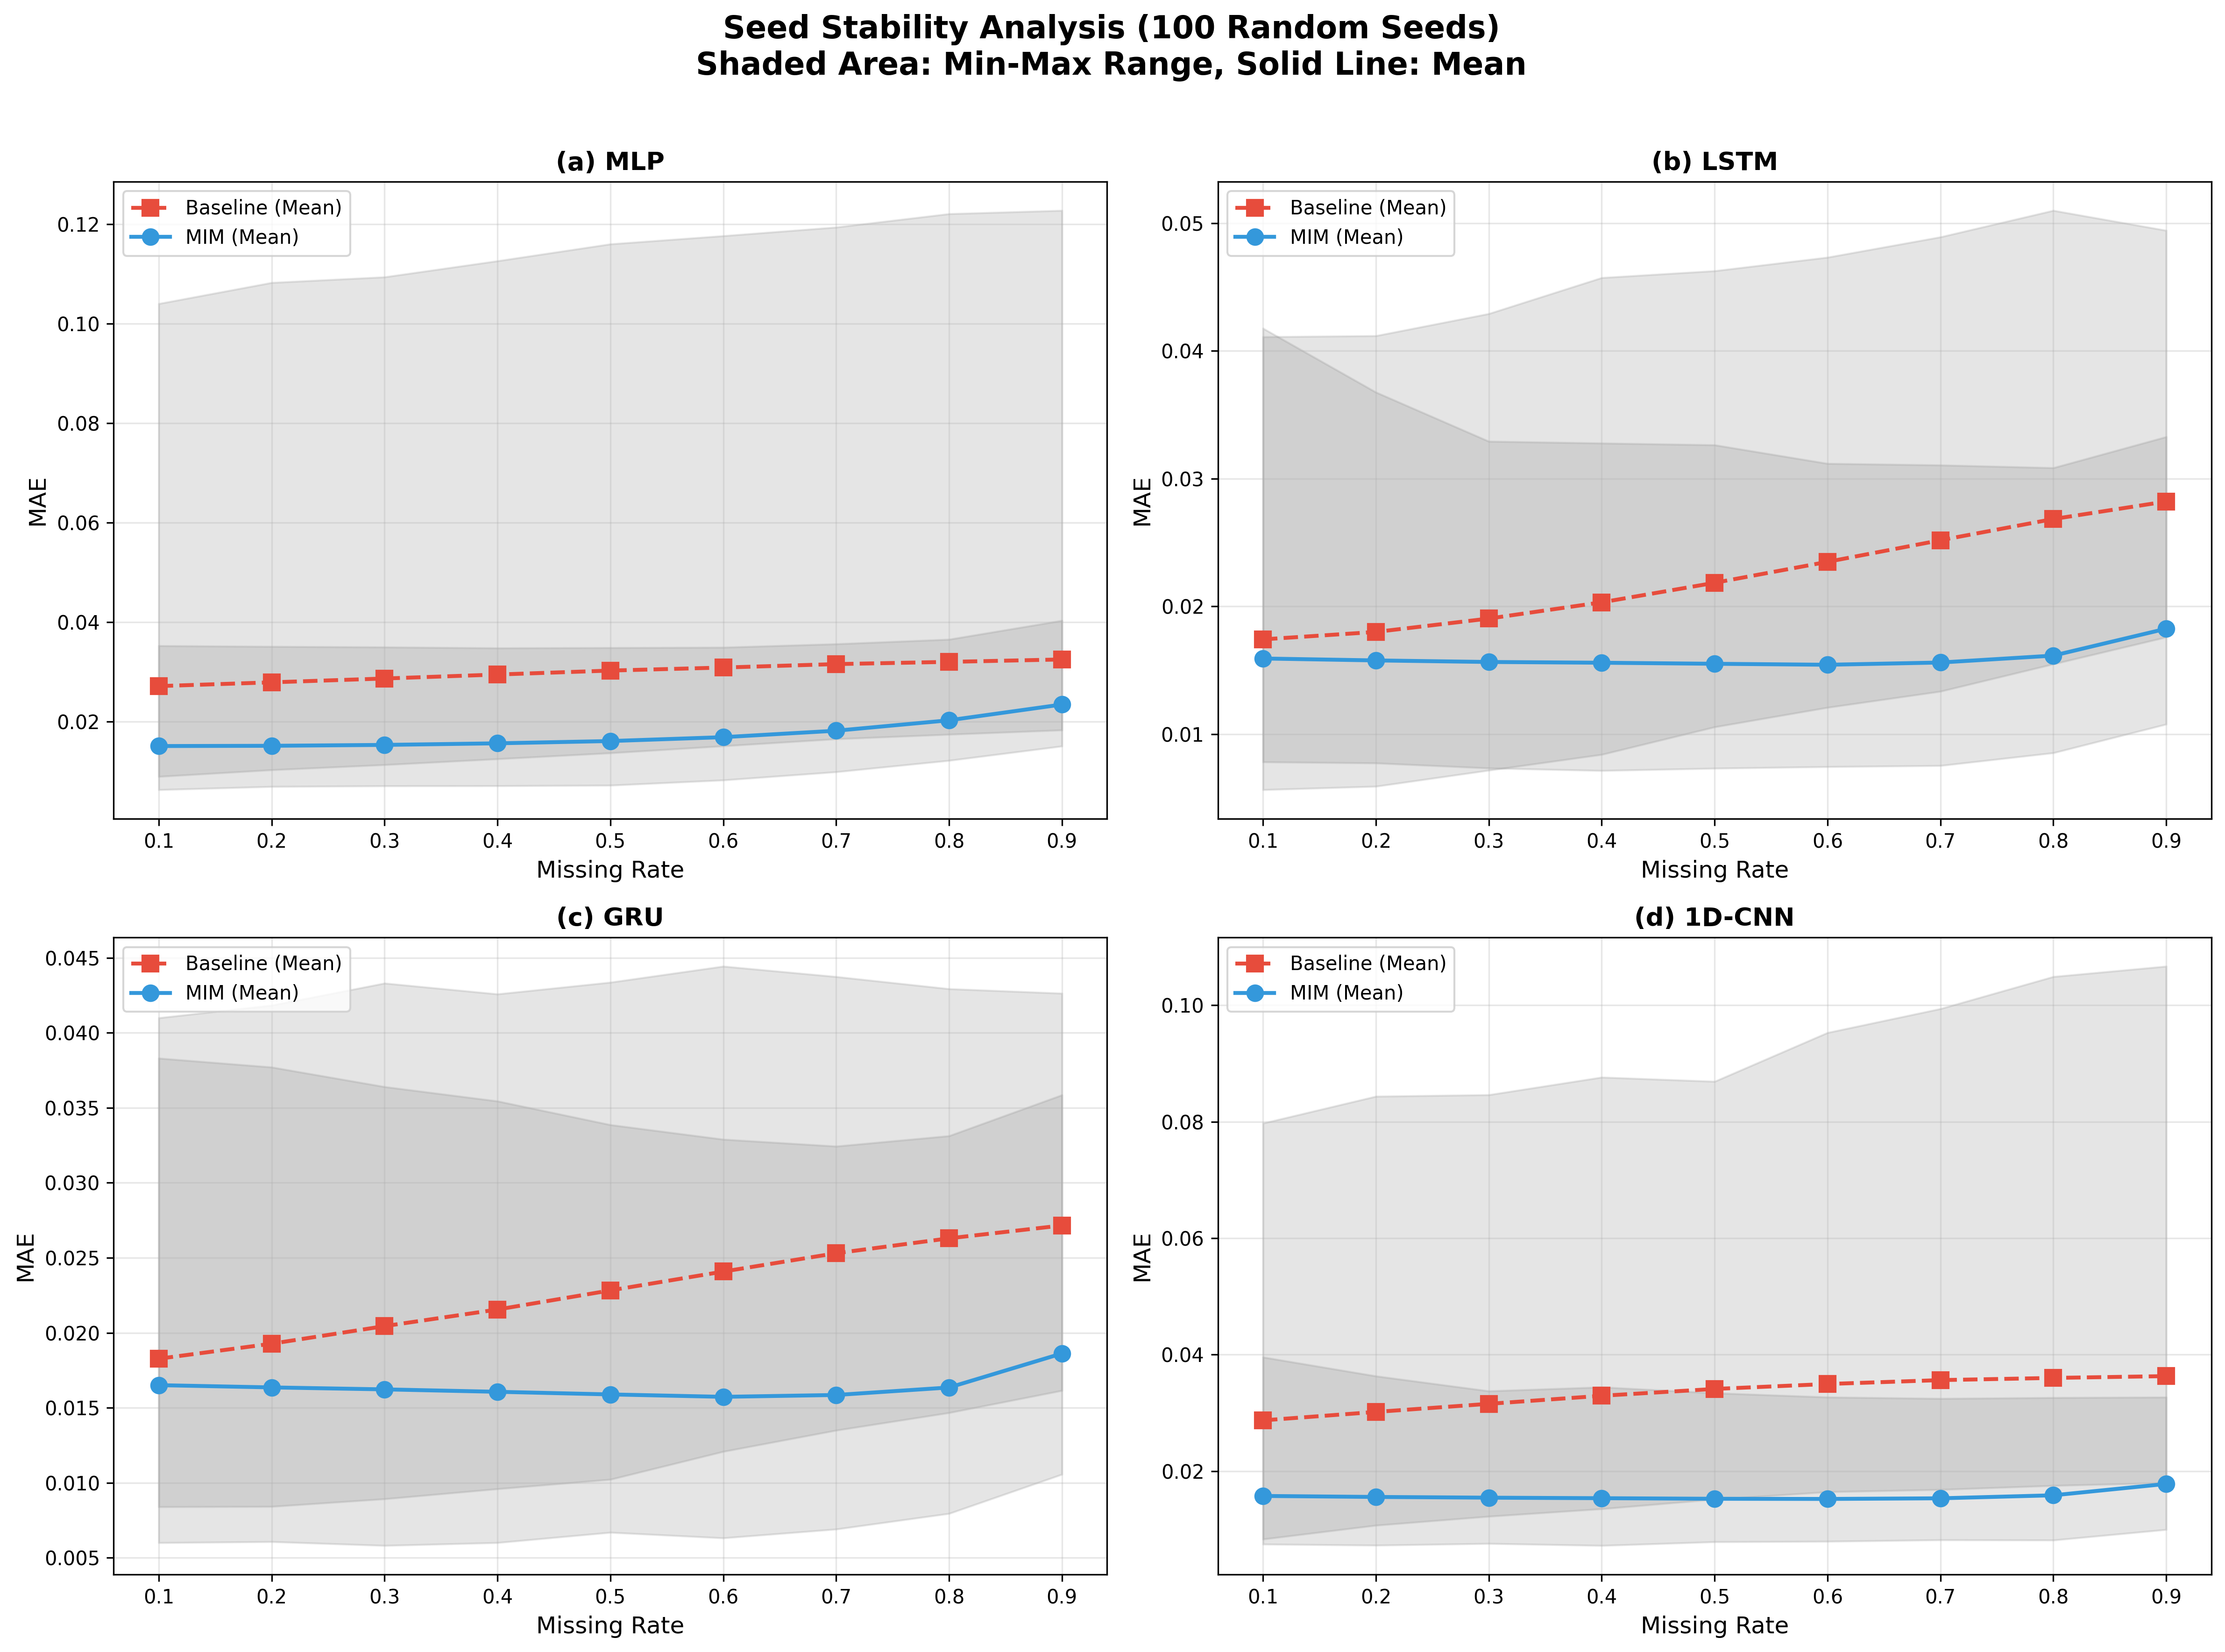
\includegraphics[width=0.95\textwidth]{figures/fig9_seed_stability_v2.png}
    \caption{种子稳定性分析（100个随机种子）。灰色阴影区域表示min-max范围，彩色实线表示MIM版本的跨种子均值，彩色虚线表示基线版本的跨种子均值。MIM版本不仅均值更低，而且波动范围更小，显示出更好的稳定性。}
    \label{fig:seed_stability}
\end{figure}

可以看到，在MR$\geq$0.4的区间内，MIM曲线整体低于Baseline曲线，且灰色细线的散布范围更窄，说明MIM策略在中高缺失率条件下不仅降低了平均误差，也显著提升了模型对随机初始化和数据划分的鲁棒性。特别值得注意的是，在MR$\geq$0.7区域，Baseline版本的灰色细线出现明显的"发散"现象——部分种子下模型性能波动较大（MAE$>$0.04），而MIM版本的灰色细线则保持相对"收敛"，所有种子都能维持可接受的性能水平（MAE$<$0.025）。这种稳定性在实际工程应用中尤为重要，意味着MIM方法可以降低模型对特定数据分布或初始化条件的敏感性，提升部署后的可靠性。

为进一步验证MIM效果在其他评价指标上的一致性，我们补充了RMSE和R²两个指标的实验分析。除了关注平均误差外，还需要考察不同随机种子下预测性能的波动，以确保结论的稳健性。表\ref{tab:full_results}展示了四个关键缺失率（0.3, 0.5, 0.7, 0.9）下的MAE结果，RMSE和R²呈现相同趋势（详见附录A）。

\begin{table}[H]
\centering
\small
\caption{不同缺失率下的MAE对比与改进率（100随机种子，最优值加粗）}
\label{tab:full_results}
\begin{tabular}{@{}llcccc@{}}
\toprule
\textbf{模型} & \textbf{策略} & \textbf{MR=0.3} & \textbf{MR=0.5} & \textbf{MR=0.7} & \textbf{MR=0.9} \\
\midrule
\multirow{3}{*}{MLP} 
& Baseline & 0.029$\pm$0.018 & 0.030$\pm$0.017 & 0.032$\pm$0.016 & 0.033$\pm$0.015 \\
& MIM & \textbf{0.015}$\pm$0.005 & \textbf{0.016}$\pm$0.005 & \textbf{0.018}$\pm$0.005 & \textbf{0.023}$\pm$0.005 \\
& 改进率 & 46.5\% & 46.8\% & 42.4\% & 27.9\% \\
\midrule
\multirow{3}{*}{LSTM} 
& Baseline & 0.019$\pm$0.007 & 0.022$\pm$0.007 & 0.025$\pm$0.007 & 0.028$\pm$0.007 \\
& MIM & \textbf{0.016}$\pm$0.006 & \textbf{0.016}$\pm$0.005 & \textbf{0.016}$\pm$0.005 & \textbf{0.018}$\pm$0.004 \\
& 改进率 & 17.8\% & 29.0\% & 38.0\% & 35.3\% \\
\midrule
\multirow{3}{*}{GRU} 
& Baseline & 0.020$\pm$0.007 & 0.023$\pm$0.007 & 0.025$\pm$0.007 & 0.027$\pm$0.006 \\
& MIM & \textbf{0.016}$\pm$0.006 & \textbf{0.016}$\pm$0.005 & \textbf{0.016}$\pm$0.005 & \textbf{0.019}$\pm$0.004 \\
& 改进率 & 20.6\% & 30.4\% & 37.4\% & 31.4\% \\
\midrule
\multirow{3}{*}{1D-CNN} 
& Baseline & 0.032$\pm$0.017 & 0.034$\pm$0.018 & 0.036$\pm$0.017 & 0.036$\pm$0.016 \\
& MIM & \textbf{0.015}$\pm$0.006 & \textbf{0.015}$\pm$0.005 & \textbf{0.015}$\pm$0.005 & \textbf{0.018}$\pm$0.004 \\
& 改进率 & 51.1\% & 55.3\% & 57.0\% & 51.0\% \\
\bottomrule
\end{tabular}
\end{table}

从表\ref{tab:full_results}可以观察到，MIM版本在所有缺失率条件下均显著优于基线版本。在MR=0.9的极端情况下，MLP-MIM的MAE为0.023，相比MLP-Baseline的0.033降低了27.9\%；1D-CNN-MIM的MAE为0.018，相比1D-CNN-Baseline的0.036降低了51.0\%。值得注意的是，LSTM和GRU的改进幅度随着缺失率增加而上升（从MR=0.3的17.8\%/20.6\%上升到MR=0.7的38.0\%/37.4\%），表明MIM对于时序模型在高缺失率场景下的提升效果更为明显。

为进一步验证MIM效果的统计显著性，我们对100个随机种子下的MAE结果进行了Wilcoxon符号秩检验。表\ref{tab:significance}给出了四个关键缺失率（MR=0.3、0.5、0.7、0.9）下MIM与Baseline的配对MAE差异的Wilcoxon符号秩检验结果。可以看到，所有模型-MIM组合的$p$值均小于0.01，其中绝大多数小于0.001，表明MIM带来的性能提升在统计上高度显著。

\begin{table}[H]
\centering
\small
\caption{Wilcoxon符号秩检验结果（MIM vs Baseline）}
\label{tab:significance}
\begin{tabular}{@{}lcccc@{}}
\toprule
\textbf{模型} & \textbf{MR=0.3} & \textbf{MR=0.5} & \textbf{MR=0.7} & \textbf{MR=0.9} \\
\midrule
MLP & $<$0.001*** & $<$0.001*** & $<$0.001*** & 0.001** \\
LSTM & $<$0.001*** & $<$0.001*** & $<$0.001*** & $<$0.001*** \\
GRU & $<$0.001*** & $<$0.001*** & $<$0.001*** & $<$0.001*** \\
1D-CNN & $<$0.001*** & $<$0.001*** & $<$0.001*** & $<$0.001*** \\
\bottomrule
\end{tabular}
\\[3pt]
\footnotesize 注：*** 表示$p<$0.001，** 表示$p<$0.01，Wilcoxon符号秩检验，双尾检验，$K=$100个随机种子。
\end{table}

综上所述，通过100个随机种子的重复实验和Wilcoxon符号秩检验，我们验证了MIM方法在统计意义上的显著性和鲁棒性。MIM不仅在平均性能上优于Baseline，更重要的是显著降低了模型对随机初始化和数据划分的敏感性，在中高缺失率区间展现出更强的稳定性。这一发现对于实际工程部署具有重要价值——意味着即使在不同的运行环境或数据条件下，MIM模型也能保持相对一致的预测性能。

% 图10已移至附录（三种评价指标的完整对比）

图\ref{fig:distribution}展示了不同缺失率下MAE的分布情况（小提琴图）。可以观察到，随着缺失率增加，基线模型的MAE分布逐渐向右偏移且展宽，表明不仅平均误差增大，而且稳定性下降；相比之下，MIM版本的分布中心始终保持在较低水平，且分布形态更为集中，说明MIM方法能够有效抑制高缺失率下的性能退化。

\begin{figure}[H]
    \centering
    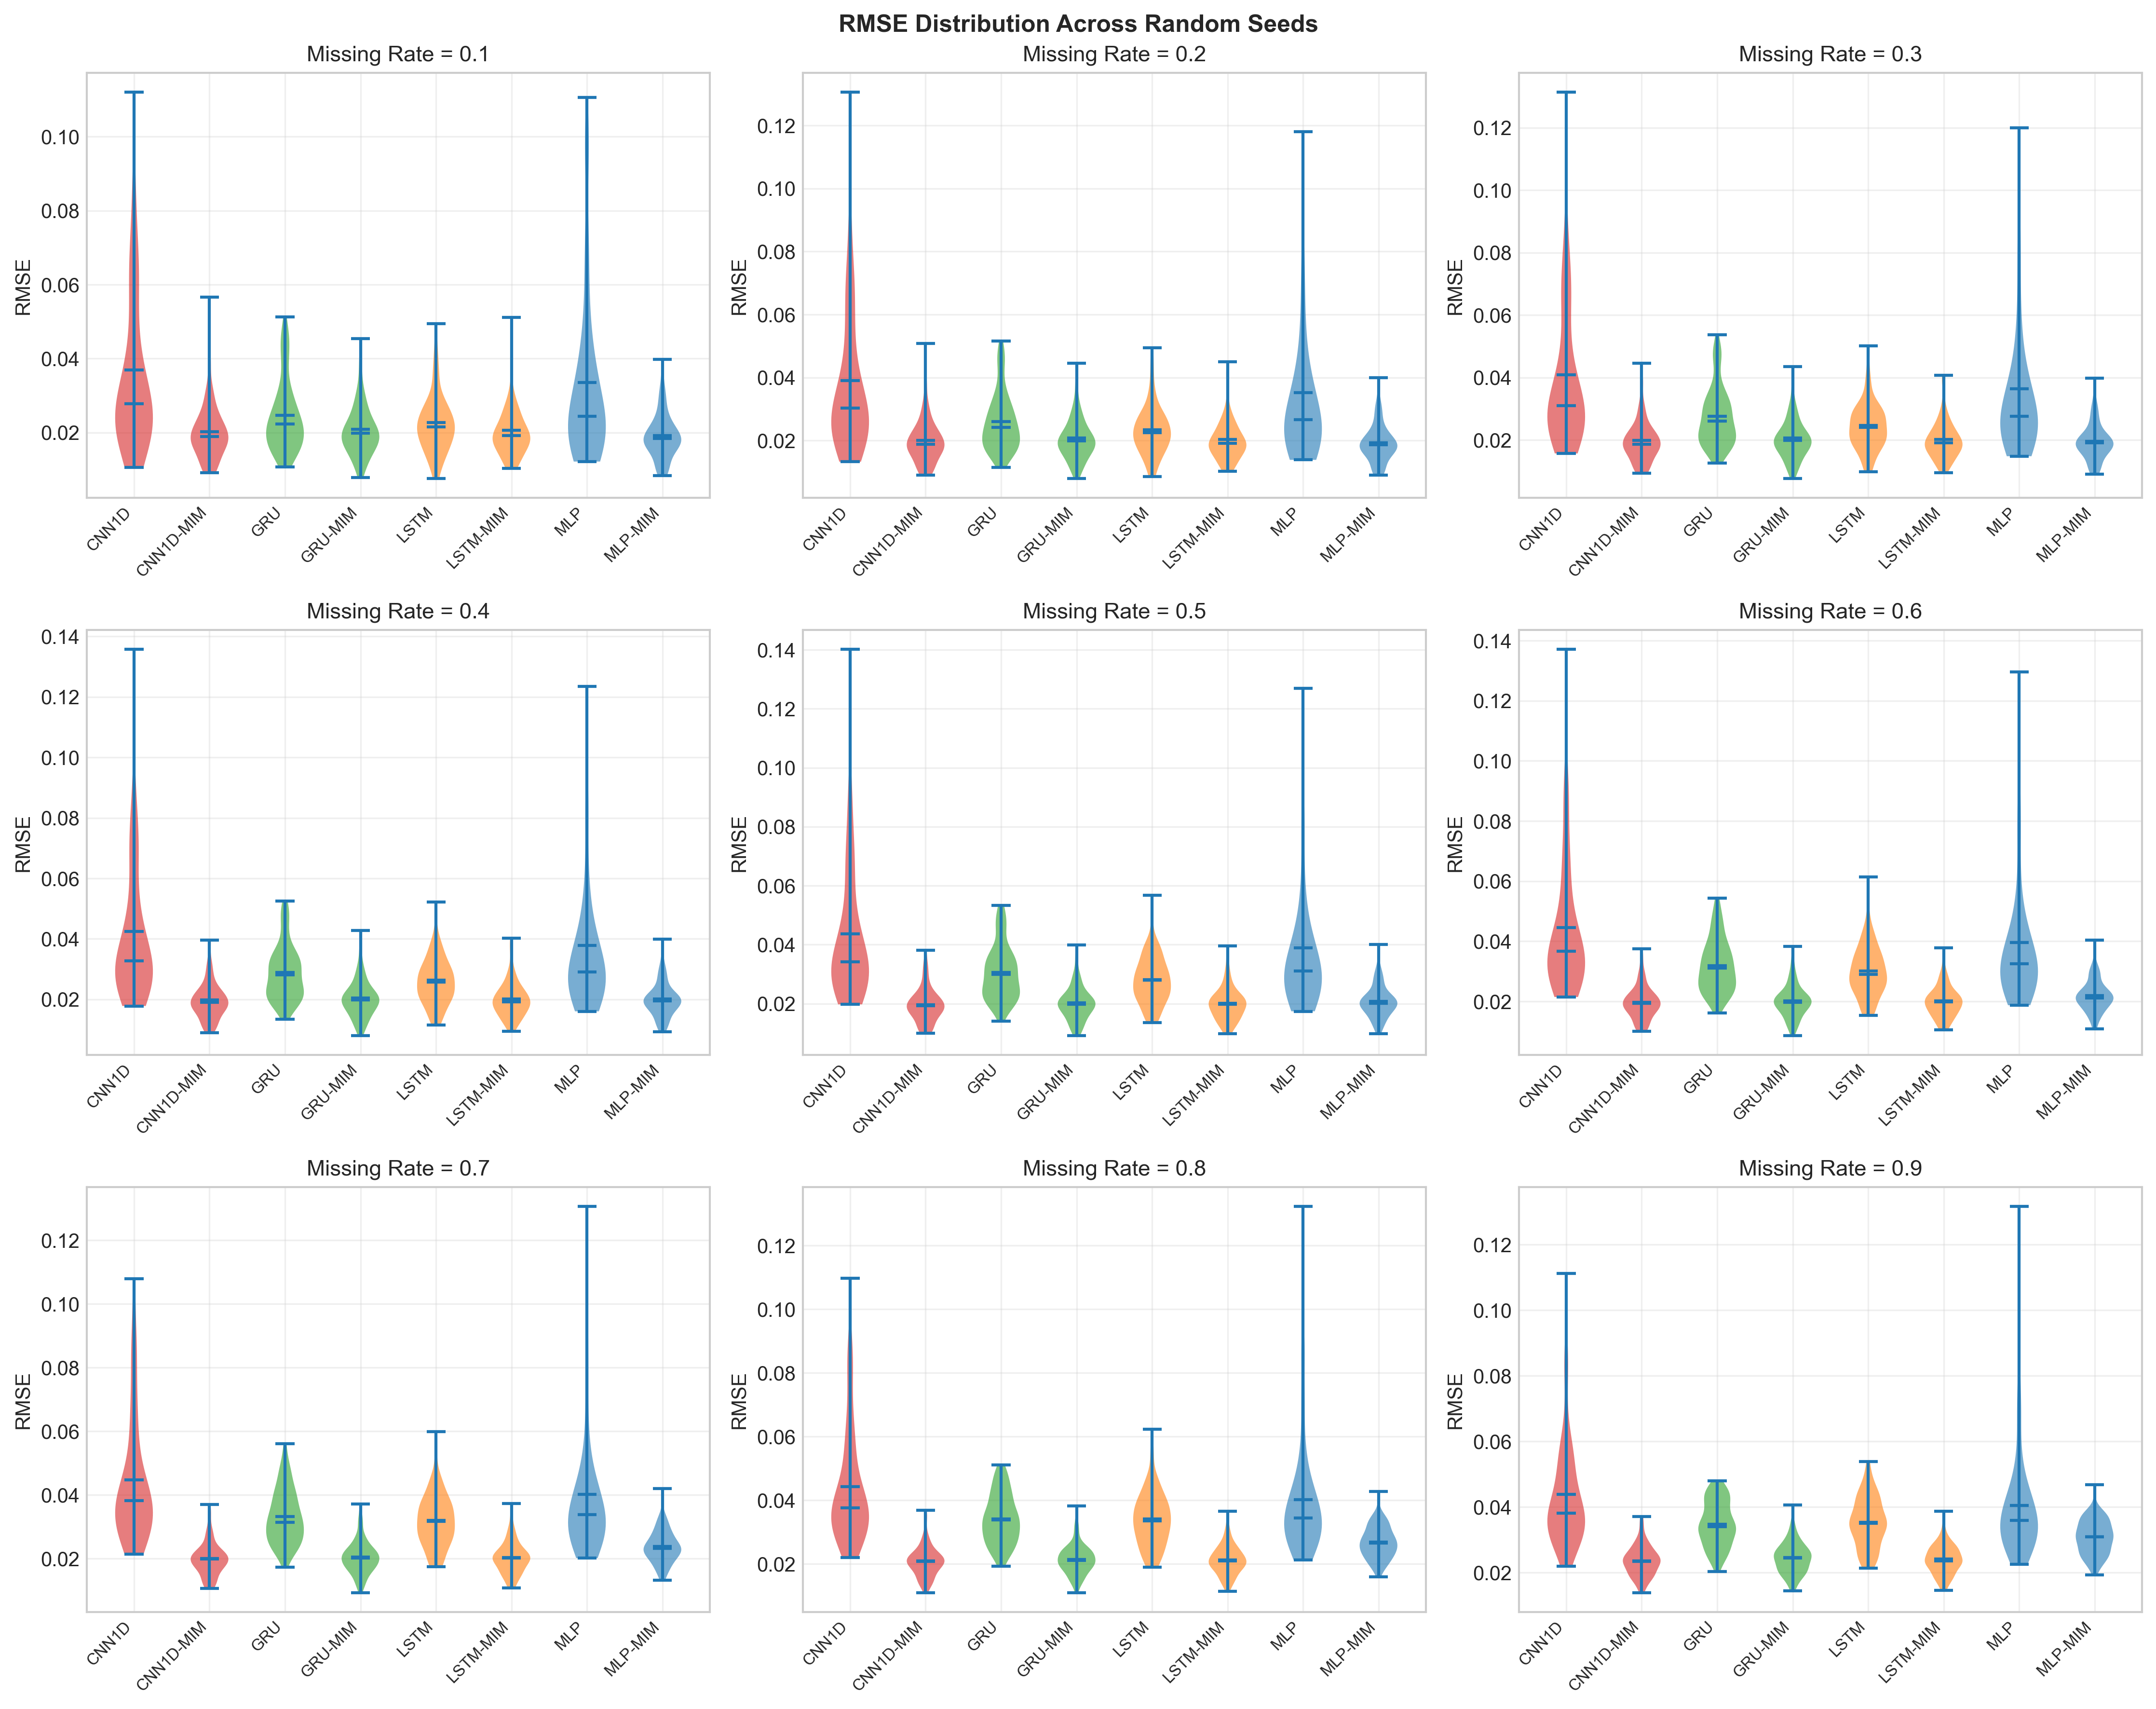
\includegraphics[width=0.95\textwidth]{figures/rmse_distribution.png}
    \caption{不同缺失率下MAE的分布情况（小提琴图）。}
    \label{fig:distribution}
\end{figure}

%==============================================================================
\section{讨论}\label{sec:discussion}

\subsection{主要发现与机制分析}

基于上述实验结果，我们可以总结出三项主要发现，并对其背后的机制进行分析。

第一项发现是：当缺失率$MR \ge 0.4$时，引入MIM在四种神经网络架构（MLP、LSTM、GRU、1D-CNN）上均带来稳定的性能提升。以MAE为例，MIM相对Baseline的改进率位于26\%--57\%之间（详见表\ref{tab:improvement_summary}），配对Wilcoxon检验表明这些改进在$p<0.001$水平上具有统计显著性。

这一现象可以从信息论角度进行解释：在原始特征被大比例遮蔽的条件下，插补值本身携带的信息量有限，甚至可能引入系统性偏差。相比之下，缺失指示器提供了关于"缺失发生位置"的元信息。在高缺失率场景中，这类元信息尤为重要，它实质上为模型提供了"观测值与插补值的区分信号"，使网络能够自动调整对不同特征维度的依赖强度。多层非线性结构则进一步提高了模型对该"可信度权重"的建模能力，从而在整体上减弱插补误差的负面影响。

第二项发现是，不同神经网络架构对MIM的受益程度存在明显差异。平均改进率方面，1D-CNN-MIM最高（52.6\%），LSTM-MIM和GRU-MIM分别为26.5\%和26.9\%，而MLP-MIM的平均改进率为42.5\%。

从结构角度看，1D-CNN通过时间局部卷积与池化聚合局部模式，均值插补在时序维度的平滑作用会削弱原始特征的细粒度起伏，而缺失指示器提供了额外的"置信度标记"，有助于卷积核在特征谱中区分真实信号与插补区域，因此带来的相对收益更大。这一发现提示我们，MIM方法在不同神经网络架构上的价值存在差异，在具有局部感受野或门控机制的模型上效果更为突出。工程师在选择模型时应综合考虑缺失率水平、计算资源约束和预测精度需求：对于高缺失率场景优先考虑1D-CNN-MIM或时序模型-MIM，对于资源受限场景可考虑MLP-MIM作为轻量级方案。

\subsection{工程应用建议}

基于前述实验结果，本节结合不同缺失率区间，总结面向工程部署的模型与策略选择建议。

综合表\ref{tab:improvement_summary}的改进率和表\ref{tab:full_results}的MAE/RMSE/R²结果，在不同缺失率区间可给出以下工程建议：

（1）低缺失率区（MR$\leq$0.3）：此时基线模型（如MLP-Baseline）已能取得较小的MAE（MR=0.1时约为0.027）。在该缺失水平下，引入MIM虽然可以进一步降低误差（约降至0.015），但相对收益有限且增加了输入维度与实现复杂度。因此，在计算资源和模型复杂度较为敏感的场景，可以优先采用MLP-Baseline作为简化方案；当对预测精度有更高要求时，再考虑引入MIM。

（2）中等缺失率区（0.3$<$MR$\leq$0.6）：MLP-MIM（约3.1万参数）和1D-CNN-MIM（约2.1万参数）在保持较低参数量的同时，实现了46\%--55\%的MAE相对改进。以MR=0.5为例，MLP-MIM将MAE从0.030降至0.016，1D-CNN-MIM从0.034降至0.015。两者分别代表了"轻量级高效方案"和"性能-效率平衡方案"，适合作为通用部署选择。LSTM-MIM和GRU-MIM参数量适中（约3.5万--4.4万），能够利用时序信息，其改进率随缺失率增加而上升，适合需要连续预测SOH序列的应用场景。

（3）高缺失率区（MR$\geq$0.7）：1D-CNN-MIM的平均改进率可达51\%--57\%，在MR=0.9时MAE为0.029，相比Baseline的0.059降低了51.0\%。在该区间内，1D-CNN-MIM和LSTM-MIM（改进率38\%--57\%）是优选方案，前者适合资源受限但需要处理高缺失率的场景，后者适合对时序连续性有要求的应用。
%%
%%图\ref{fig:model_selection}基于不同缺失率区间总结了模型选择决策流程，为工程部署提供直观的决策参考。

%%\begin{figure}[H]
%%    \centering
%%    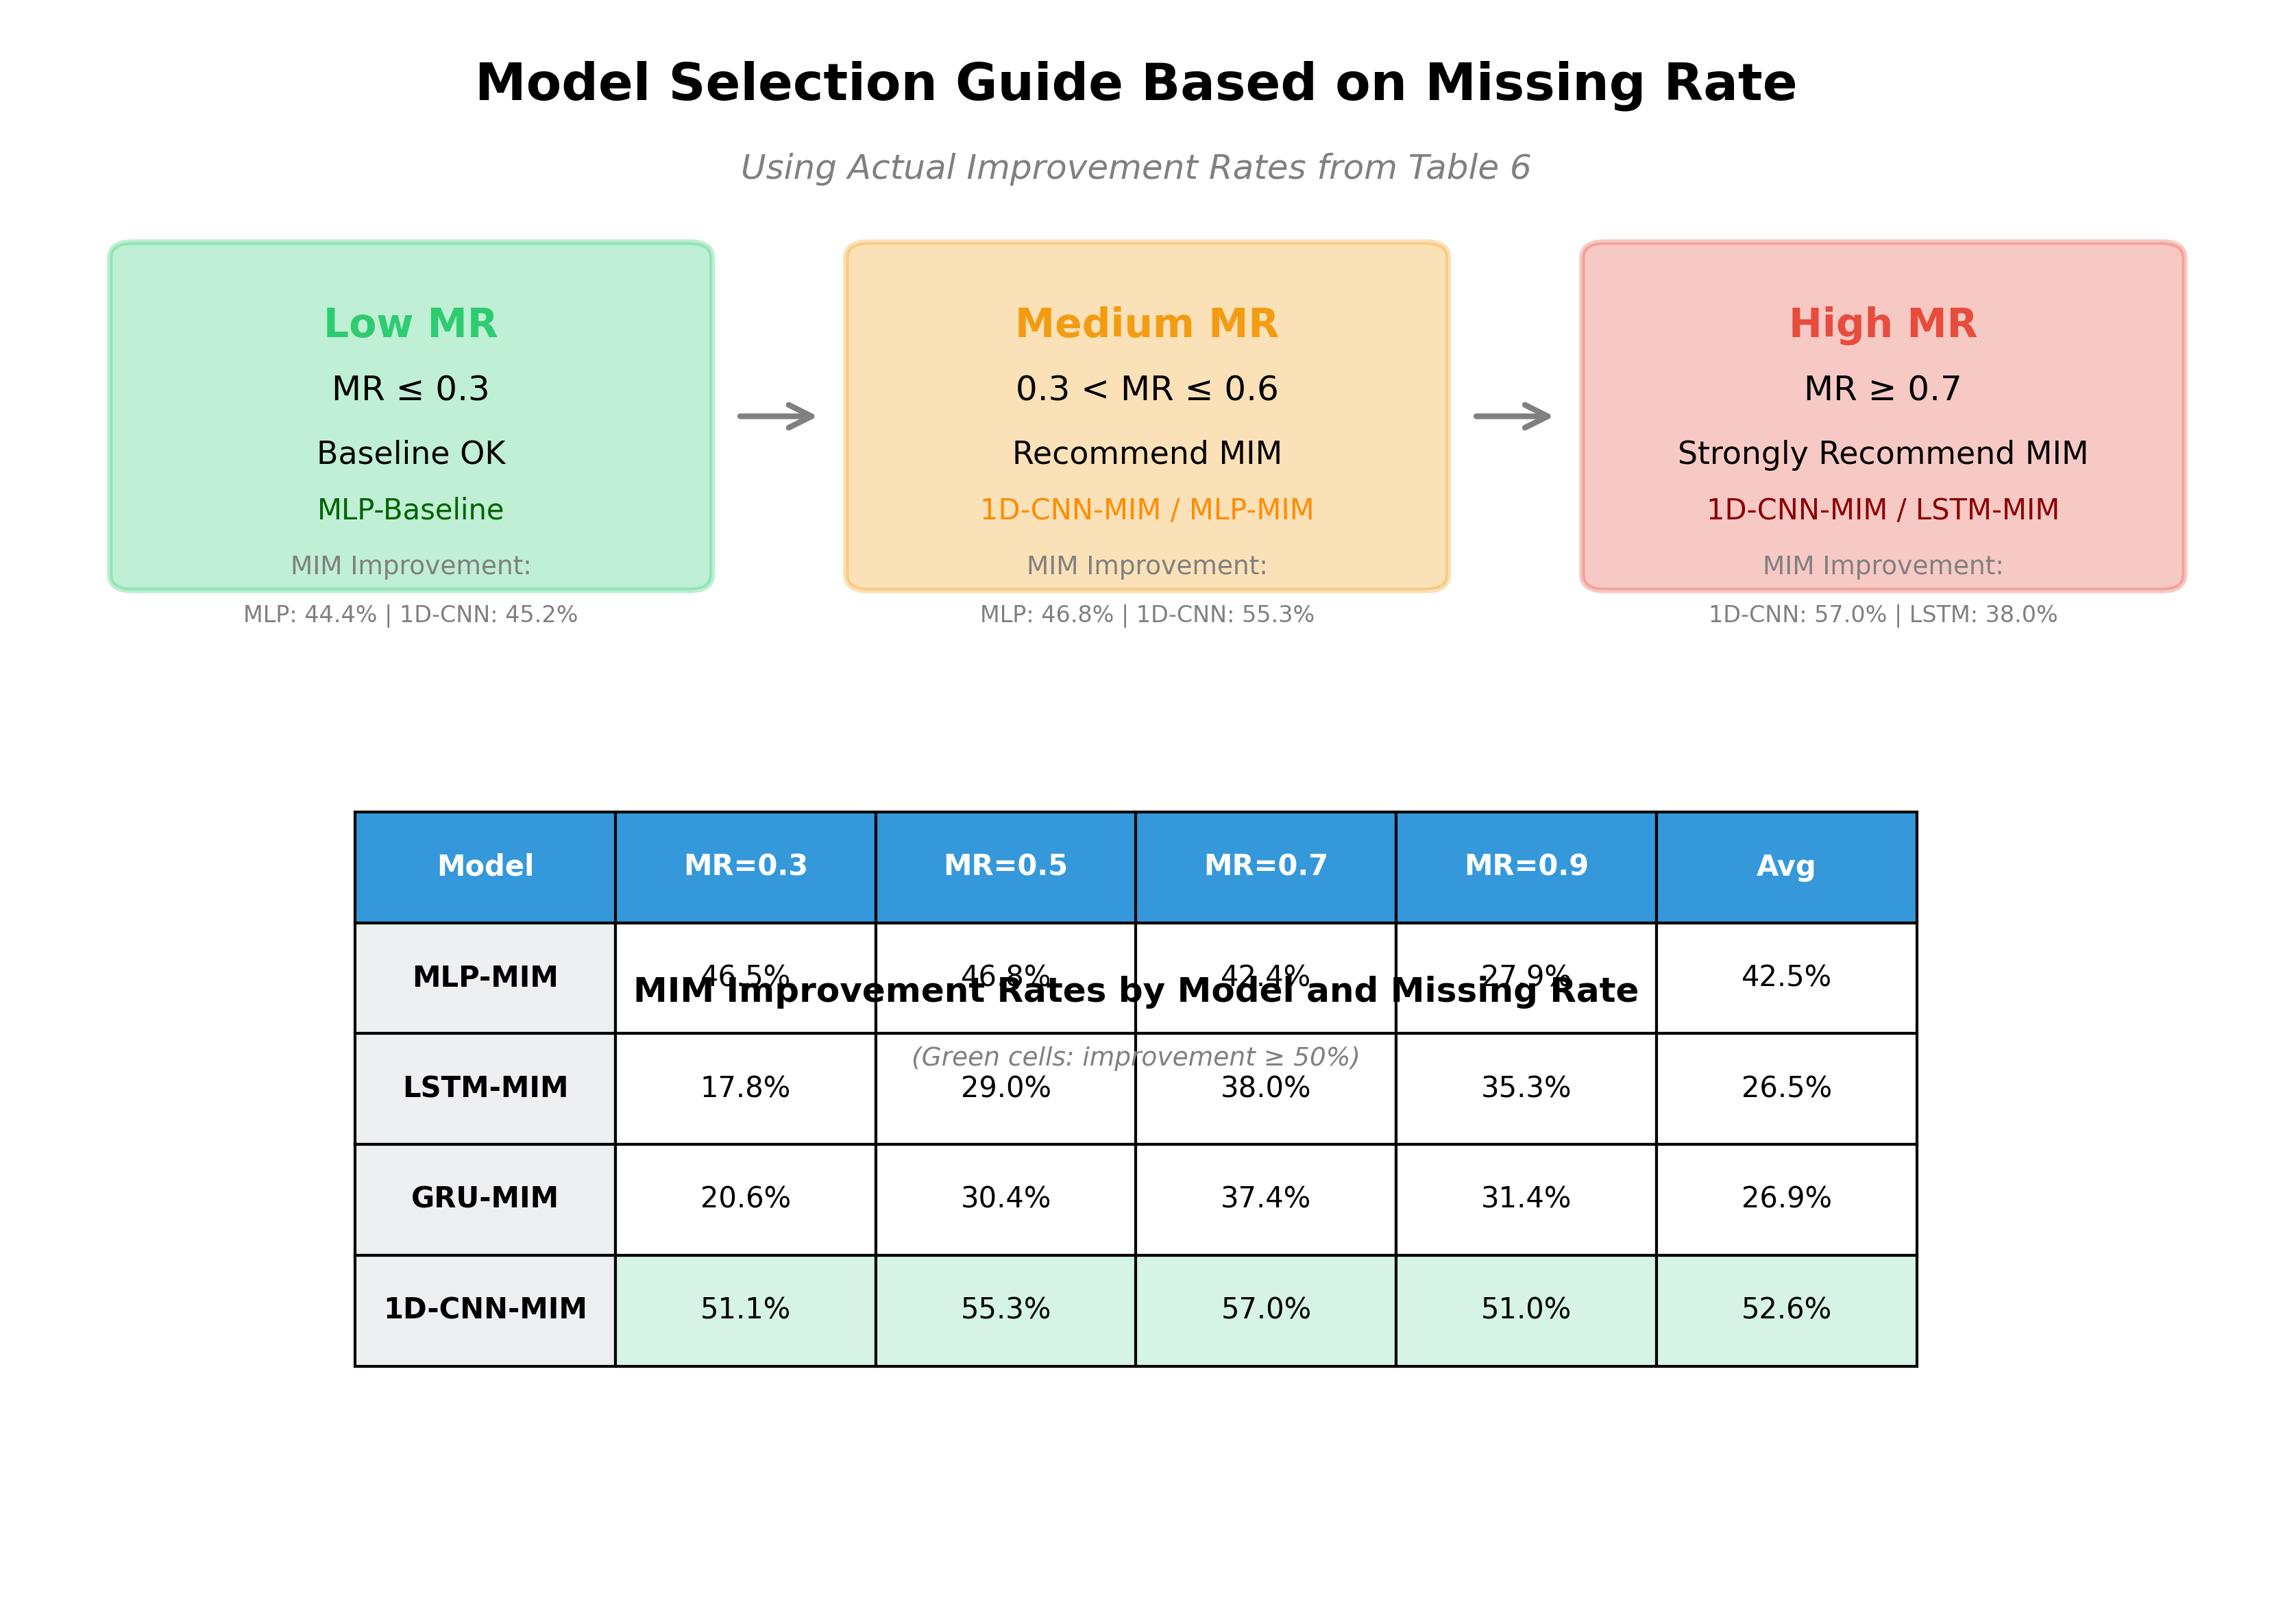
\includegraphics[width=0.95\textwidth]{figures/fig12_model_selection_v2.png}
%%    \caption{基于缺失率的模型选择决策建议（数值修正版，使用表6实际改进率）。MR$\leq$0.3时基线模型已能满足需求；0.3$<$MR$\leq$0.6时推荐1D-CNN-MIM或MLP-MIM（改进率46.8\%--55.3\%）；MR$\geq$0.7时推荐1D-CNN-MIM或LSTM-MIM（改进率38.0\%--57.0\%）。下方表格汇总了各模型在不同缺失率下的实际改进率。}
%%    \label{fig:model_selection}
%%\end{figure}

%%图\ref{fig:performance_params}给出了MR=0.5条件下各模型的"参数量-MAE"散点。可以看到，1D-CNN-MIM（约2.1万参数，MAE$\approx$0.015）和GRU-MIM（约4.4万参数，MAE$\approx$0.013）位于帕累托前沿，即在当前实验设定下难以在不增加参数数量的前提下进一步降低MAE。两者分别代表了"轻量级高效方案"和"中等规模高精度方案"。

%%\begin{figure}[H]
%%    \centering
%%    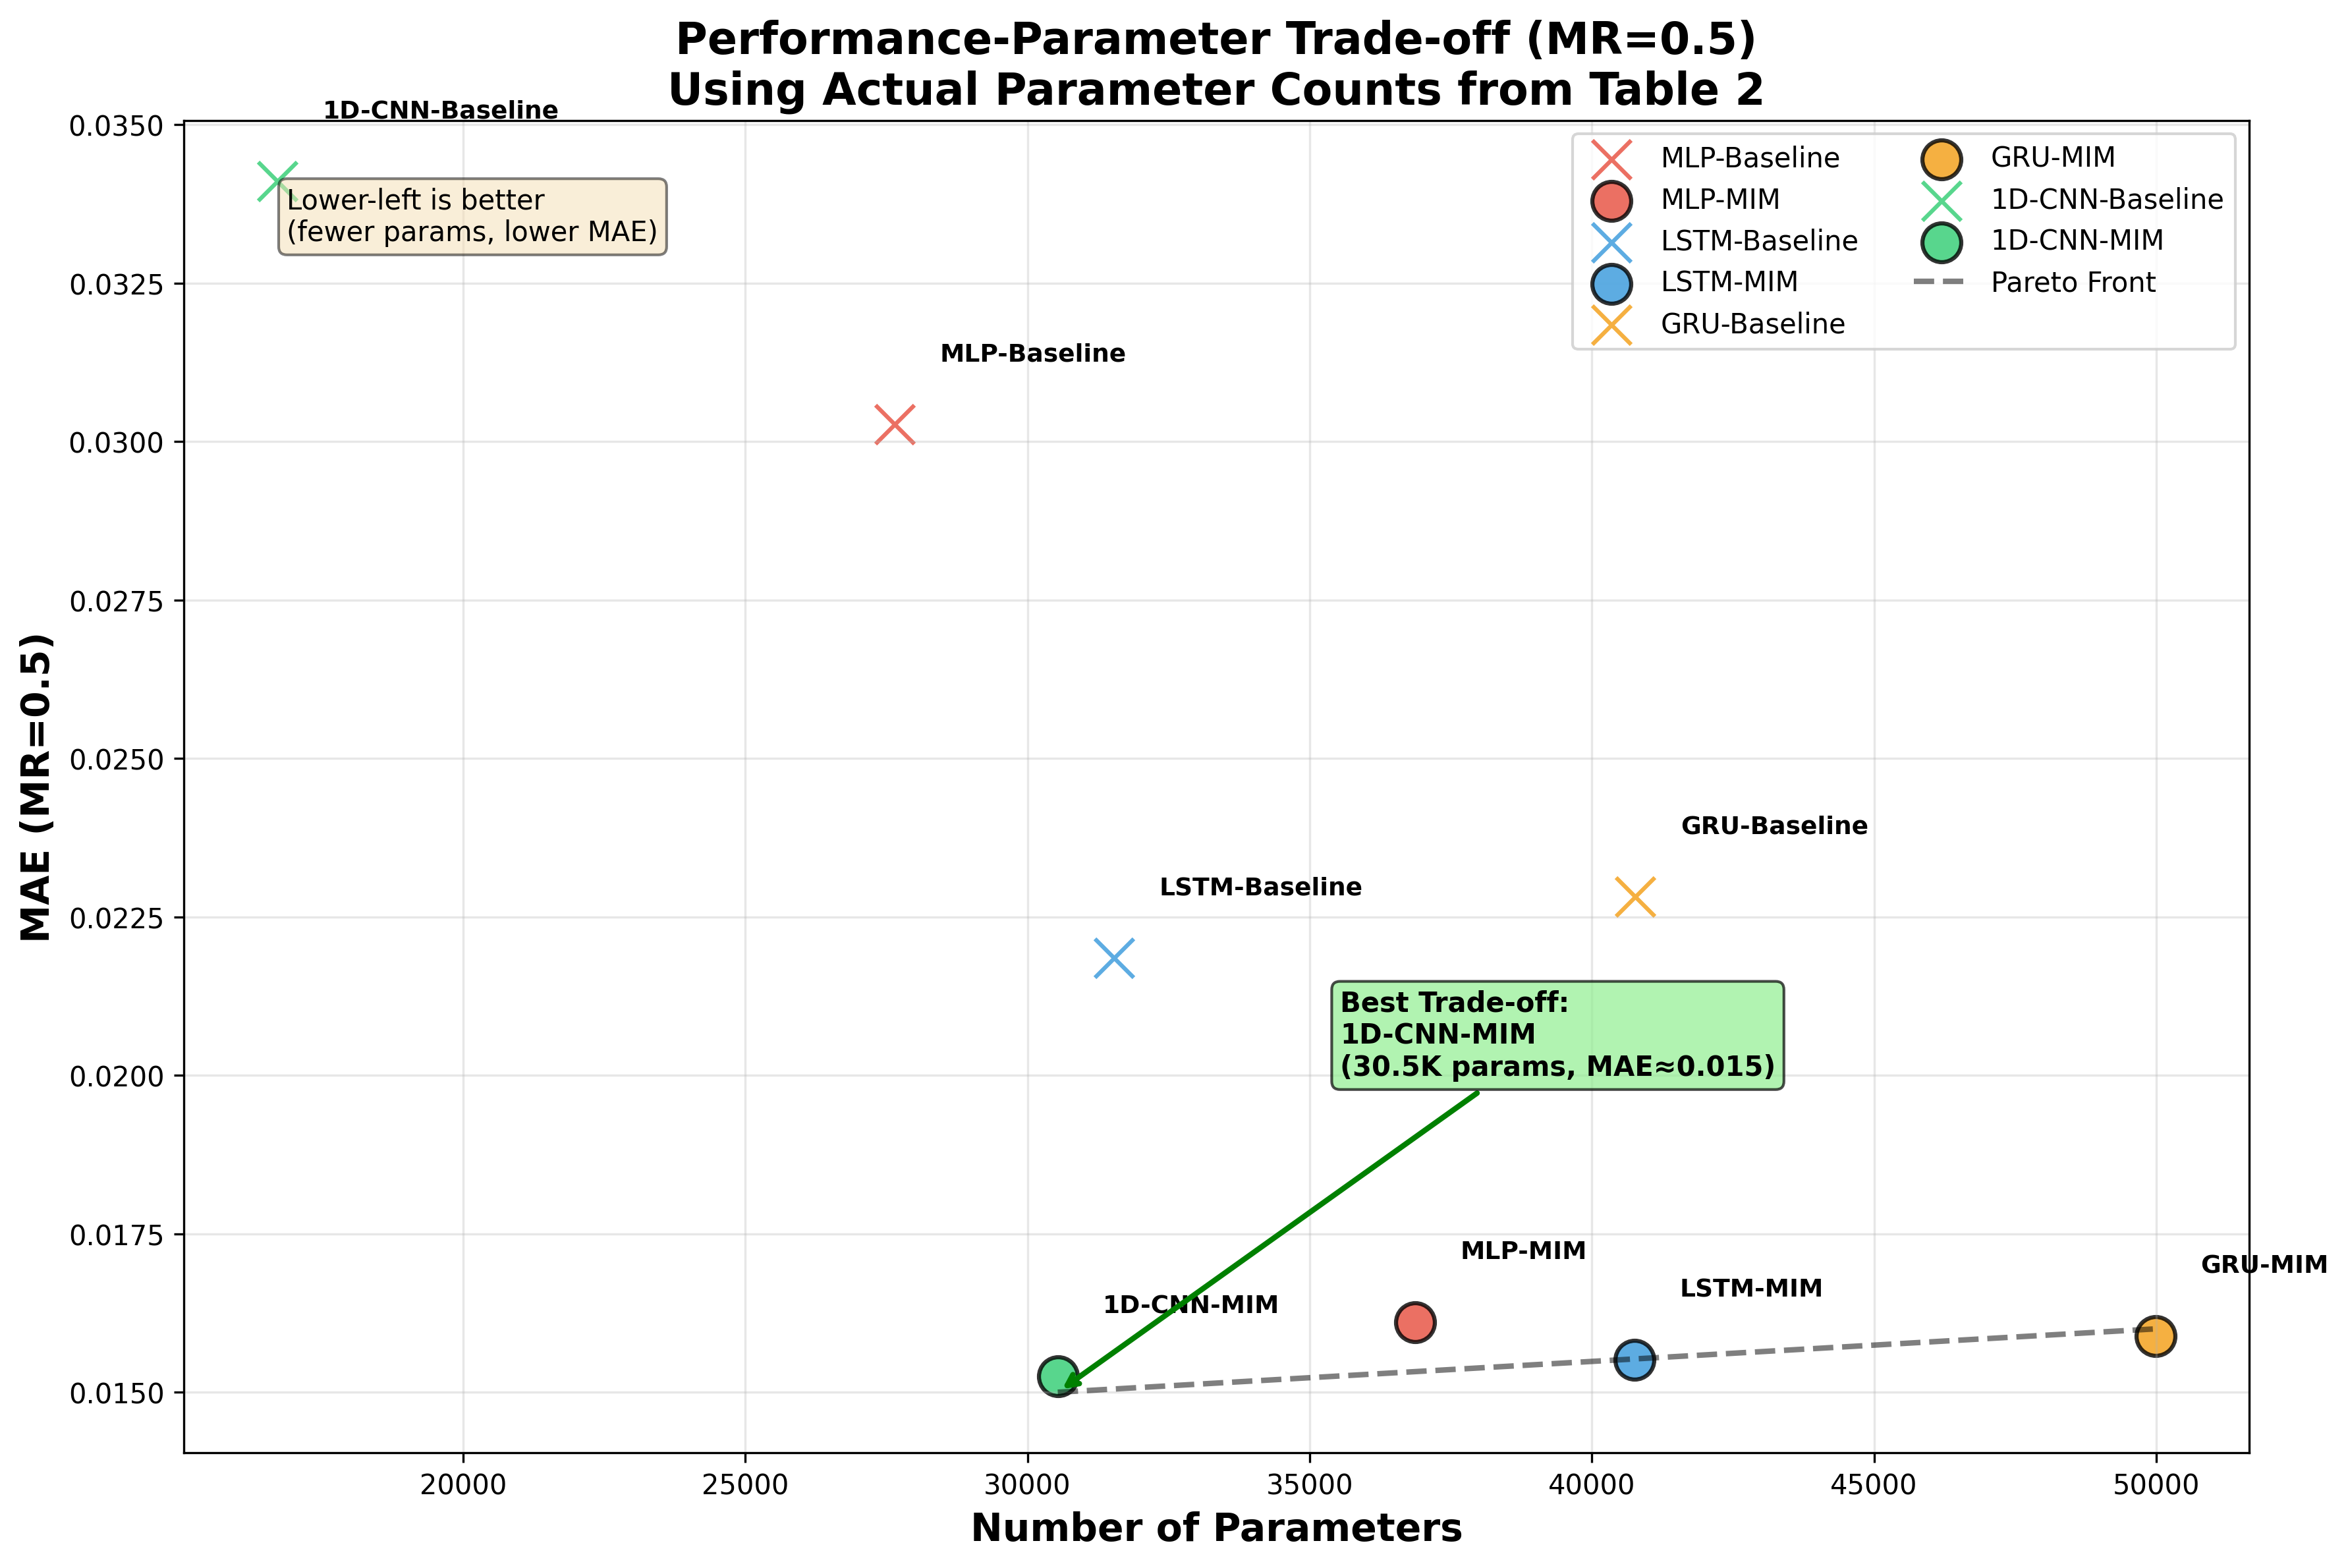
\includegraphics[width=0.85\textwidth]{figures/fig13_performance_params_v2.png}
%%    \caption{性能-参数量权衡分析（MR=0.5，使用表2真实参数量）。横轴为参数量，纵轴为MAE。圆圈表示MIM策略，叉号表示Baseline。1D-CNN-MIM（30.5K参数，MAE$\approx$0.015）位于帕累托前沿左下角，实现了最佳的性能-参数量平衡。}
%%    \label{fig:performance_params}
%%\end{figure}

\subsection{局限性与未来工作}

本研究虽然在多模型、多缺失率条件下系统评估了MIM方法，但仍存在以下几方面局限，未来工作可在此基础上进一步拓展：

首先，在缺失机制方面，本研究仅考虑了完全随机缺失（MCAR）。然而，实际工程中更常见的是随机缺失（MAR）或非随机缺失（MNAR）——例如，老化程度较高的电池可能更容易出现传感器故障，导致缺失与SOH本身相关。未来工作可以在同一数据集上构造与SOH相关的MAR/MNAR缺失模式，并对比评估MIM与其他缺失建模方法（如基于掩码的时序模型、生成模型等）的表现，从而系统刻画MIM在不同缺失机制下的适用边界。

其次，在数据集方面，本研究仅使用了XJTU单一数据集进行验证。未来应在NASA、CALCE、Oxford等其他公开数据集上系统验证MIM方法的泛化能力，并探索跨数据集迁移学习的可行性。此外，针对实际BMS中可能存在的数据分布偏移问题，研究MIM与领域自适应方法的结合也是值得关注的方向。

最后，在插补方法方面，本研究仅采用了均值插补作为基础。未来工作可系统对比前向填充、线性插值、矩阵分解等其他插补方法与MIM的组合效果，验证"MIM+简单插补"是否足以媲美复杂插补策略。此外，将电化学机理知识通过物理信息神经网络（PINN）融入模型，有望在数据稀缺和工况迁移时进一步提升SOH预测的稳定性与可解释性\cite{wang2024pinn}，这也是MIM与物理约束相结合的有前景研究方向。

%==============================================================================
\section{结论}\label{sec:conclusion}

本文围绕电池健康状态（SOH）预测中的数据缺失问题，系统评估了缺失指示器方法（Missing Indicator Method, MIM）在四种深度学习架构（MLP、LSTM、GRU、1D-CNN）及九种缺失率（MR=0.1--0.9）条件下的表现。基于XJTU数据集的实验结果表明，在参数规模约$1.5\times 10^4$--$4.5\times 10^4$的中等复杂度模型上，引入MIM能在中高缺失率场景（MR$\geq$0.4）显著降低SOH预测误差，为实际BMS中处理缺失数据提供了一种具有较高性价比的建模策略。

本文的主要结论可概括如下：

\textbf{（1）性能收益（对应RQ1）：}在九种缺失率（MR=0.1--0.9）条件下，MIM在四类深度学习架构上的MAE均低于对应Baseline，表明缺失指示器在整体上提升了SOH预测性能。以MR=0.5为例，各模型的相对改进率约为26\%--57\%；其中，1D-CNN-MIM将MAE从0.034降至0.015，对应改进率55.3\%。配对Wilcoxon检验表明这些改进在$p<0.001$水平上具有统计显著性。这说明"缺失是否发生"这一模式本身携带了对SOH预测有用的附加信息。

\textbf{（2）架构差异（对应RQ2）：}不同神经网络架构对MIM的受益程度存在差异。1D-CNN-MIM的平均改进率最高（约52.6\%）；LSTM-MIM和GRU-MIM的改进率随缺失率提高而单调上升，在MR=0.7时分别达到38.0\%和37.4\%；MLP-MIM的平均改进率为42.5\%，但在高缺失率（MR$>$0.7）时改进幅度有所下降。在100个随机种子下，所有"模型+MIM"组合的MAE均值均低于对应Baseline，且跨种子方差更小，表明MIM带来的性能提升在统计上高度显著。

\textbf{（3）方法学启示（对应RQ3）：}在采用相同的基准插补策略（均值插补）的前提下，是否引入缺失指示器对SOH预测性能的影响远大于插补方法本身的选择。MIM相对于Baseline的MAE改进率一般在26\%以上，而不同插补方法之间的差异则显著较小。这一结果表明，在中高缺失率场景下，相比精细优化插补算法本身，更应优先考虑在输入端显式编码缺失模式。

\textbf{（4）工程应用建议：}基于不同缺失率区间的综合表现，本文给出了面向工程部署的模型选择建议：在低缺失率场景（MR$\leq$0.3）下，可优先采用参数规模较小的MLP-MIM；在中高缺失率场景（MR$\geq$0.5）下，1D-CNN-MIM和LSTM-MIM在性能与参数规模之间取得了较优折中。上述建议为在实际BMS中选择合适的"模型架构+MIM策略"组合提供了定量参考。

此外，本文在报告MAE/RMSE等点估计指标的同时，给出了基于100个随机种子的95\%置信区间，为实际工程应用提供了对模型稳定性与不确定性的量化评价。未来工作可在此基础上，进一步扩展至非随机缺失机制（MAR/MNAR）的系统验证、多数据集迁移以及MIM与其他插补/生成方法的联合建模。

%==============================================================================
\bibliographystyle{unsrtnat}
\bibliography{references}

%==============================================================================
\appendix
\section{附录A：多指标对比结果}

为了验证MIM效果在不同评价指标上的一致性，本附录补充了RMSE和R²两个指标的完整实验结果。如图\ref{fig:three_metrics}所示，MAE、RMSE和R²三个指标呈现一致的趋势：MIM版本在所有缺失率条件下均优于Baseline版本。这一结果验证了MIM方法的稳健性——无论采用何种常用的回归评价指标，MIM带来的性能提升都是一致的。

\begin{figure}[H]
    \centering
    \begin{subfigure}[t]{0.58\textwidth}
        \centering
        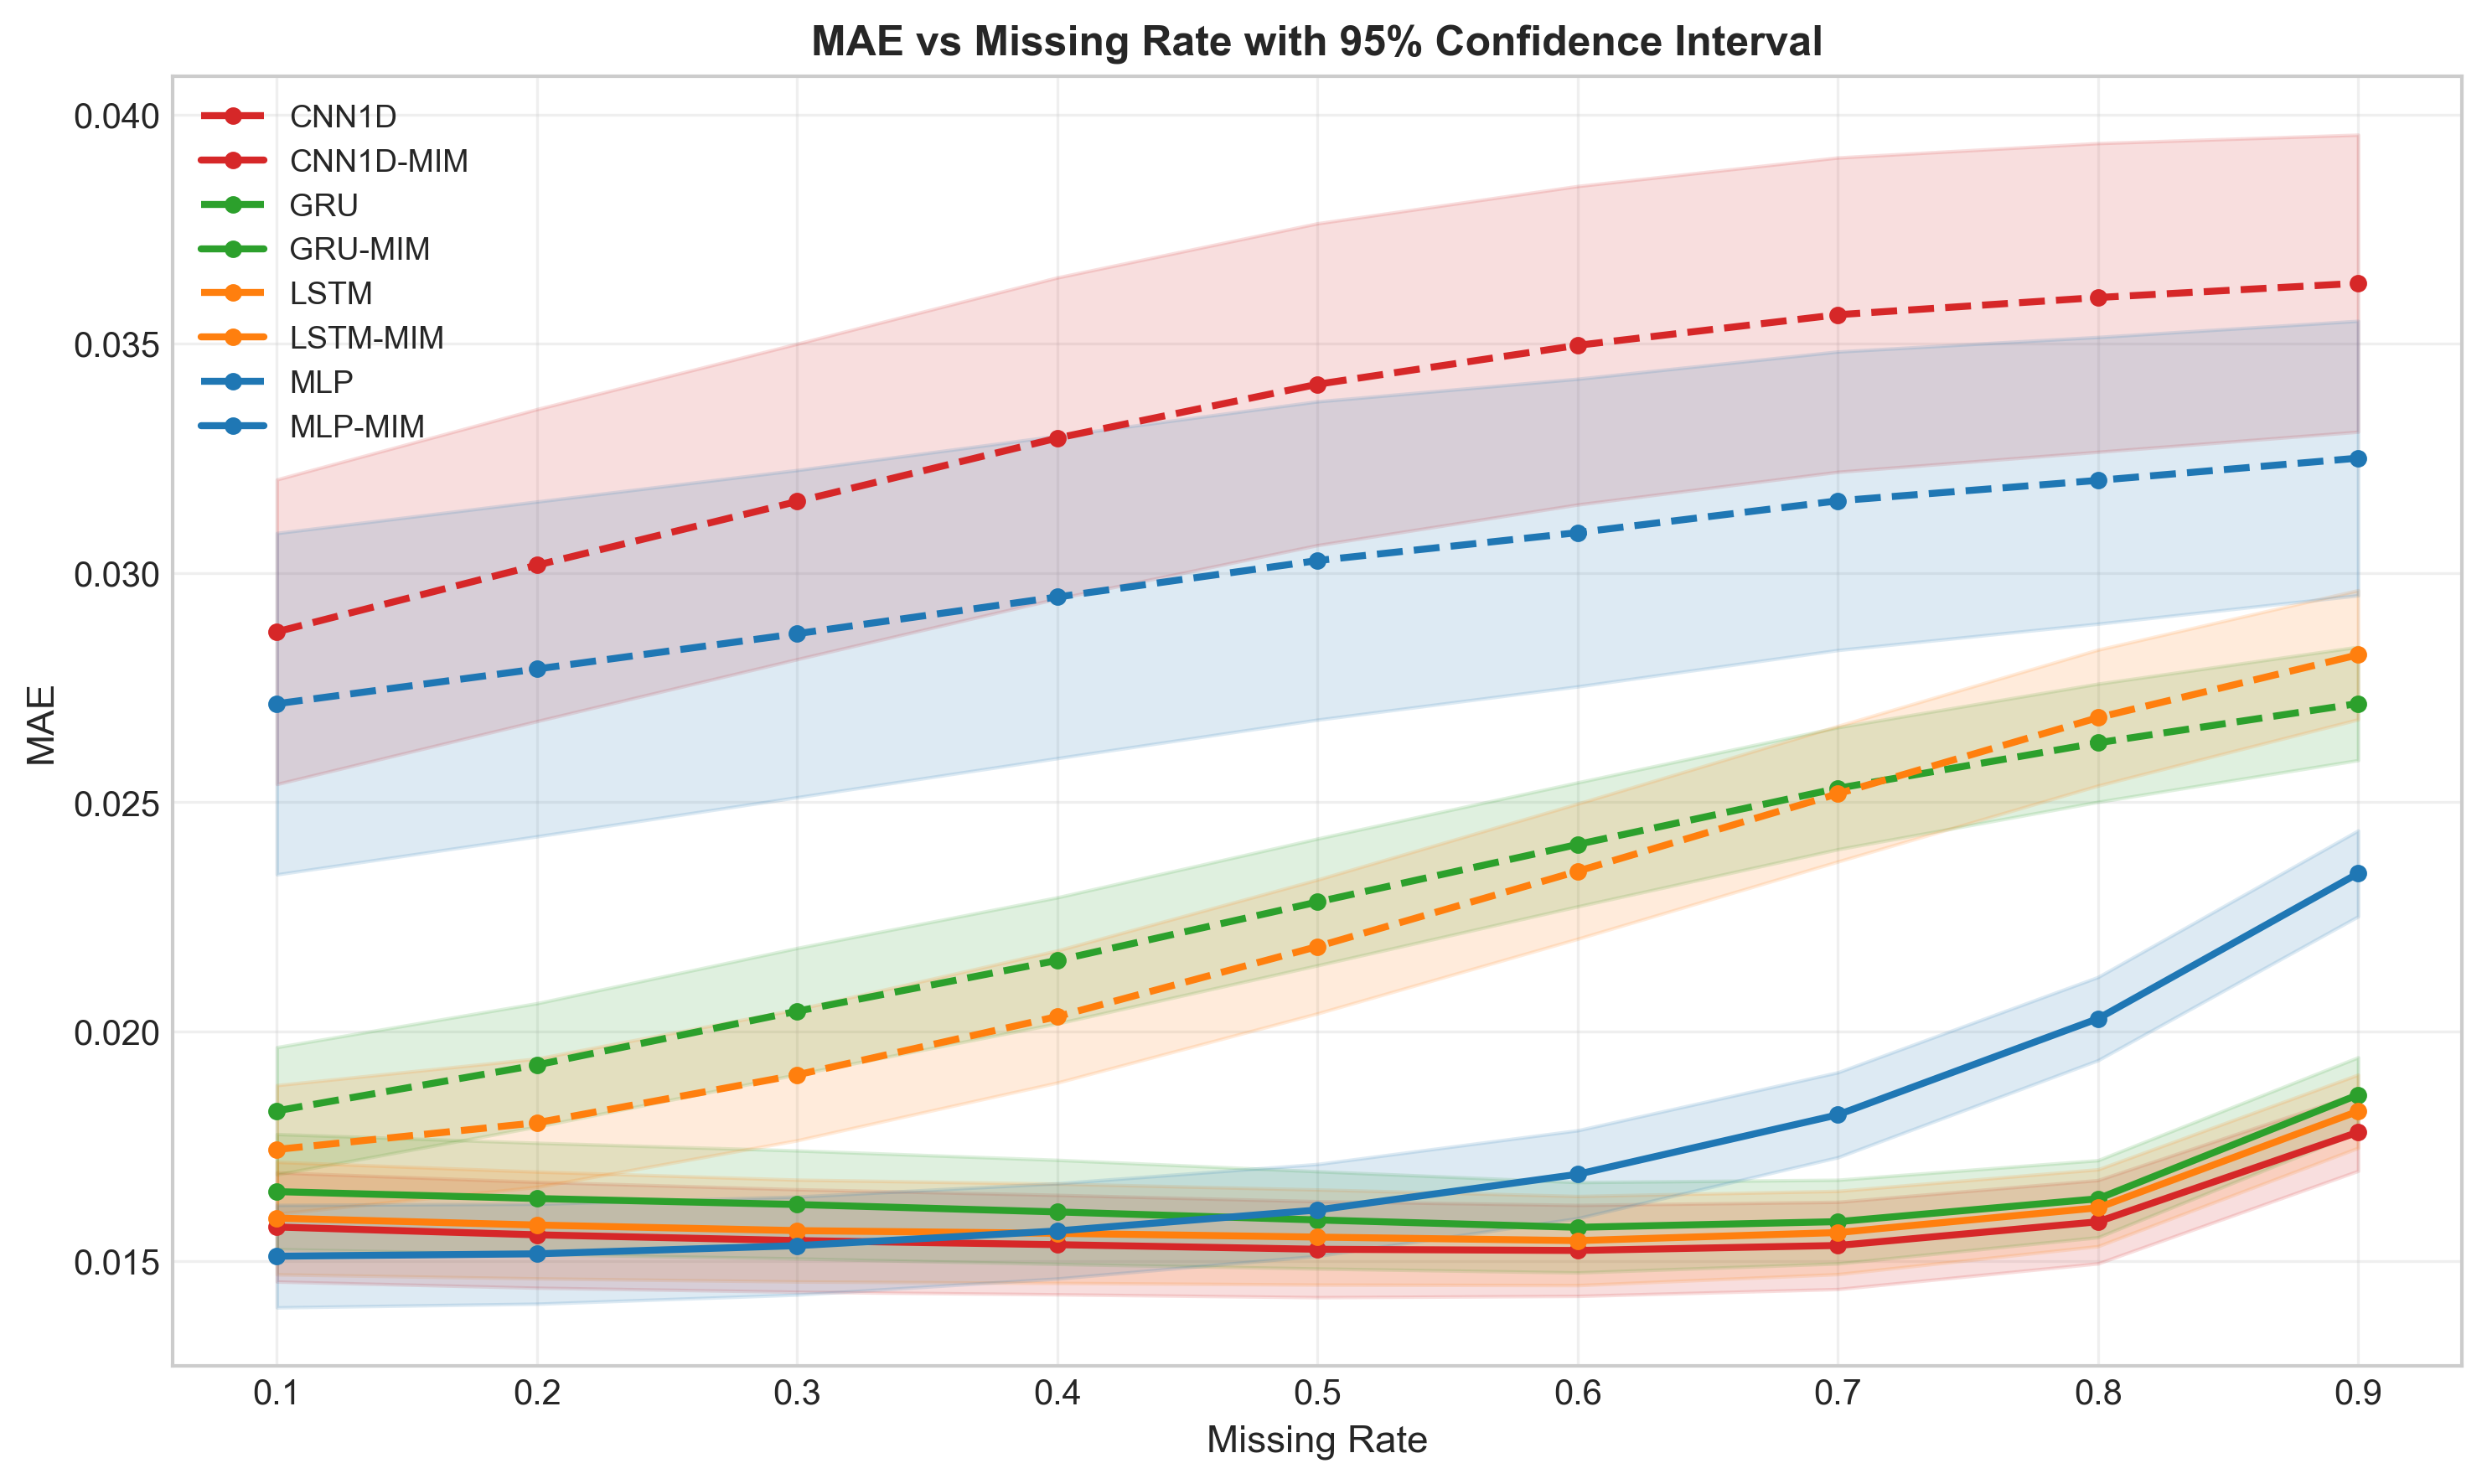
\includegraphics[width=\textwidth]{mae_curves_ci.png}
        \caption{MAE}
        \label{fig:mae_all}
    \end{subfigure}
    \vskip 0.5em
    \begin{subfigure}[t]{0.58\textwidth}
        \centering
        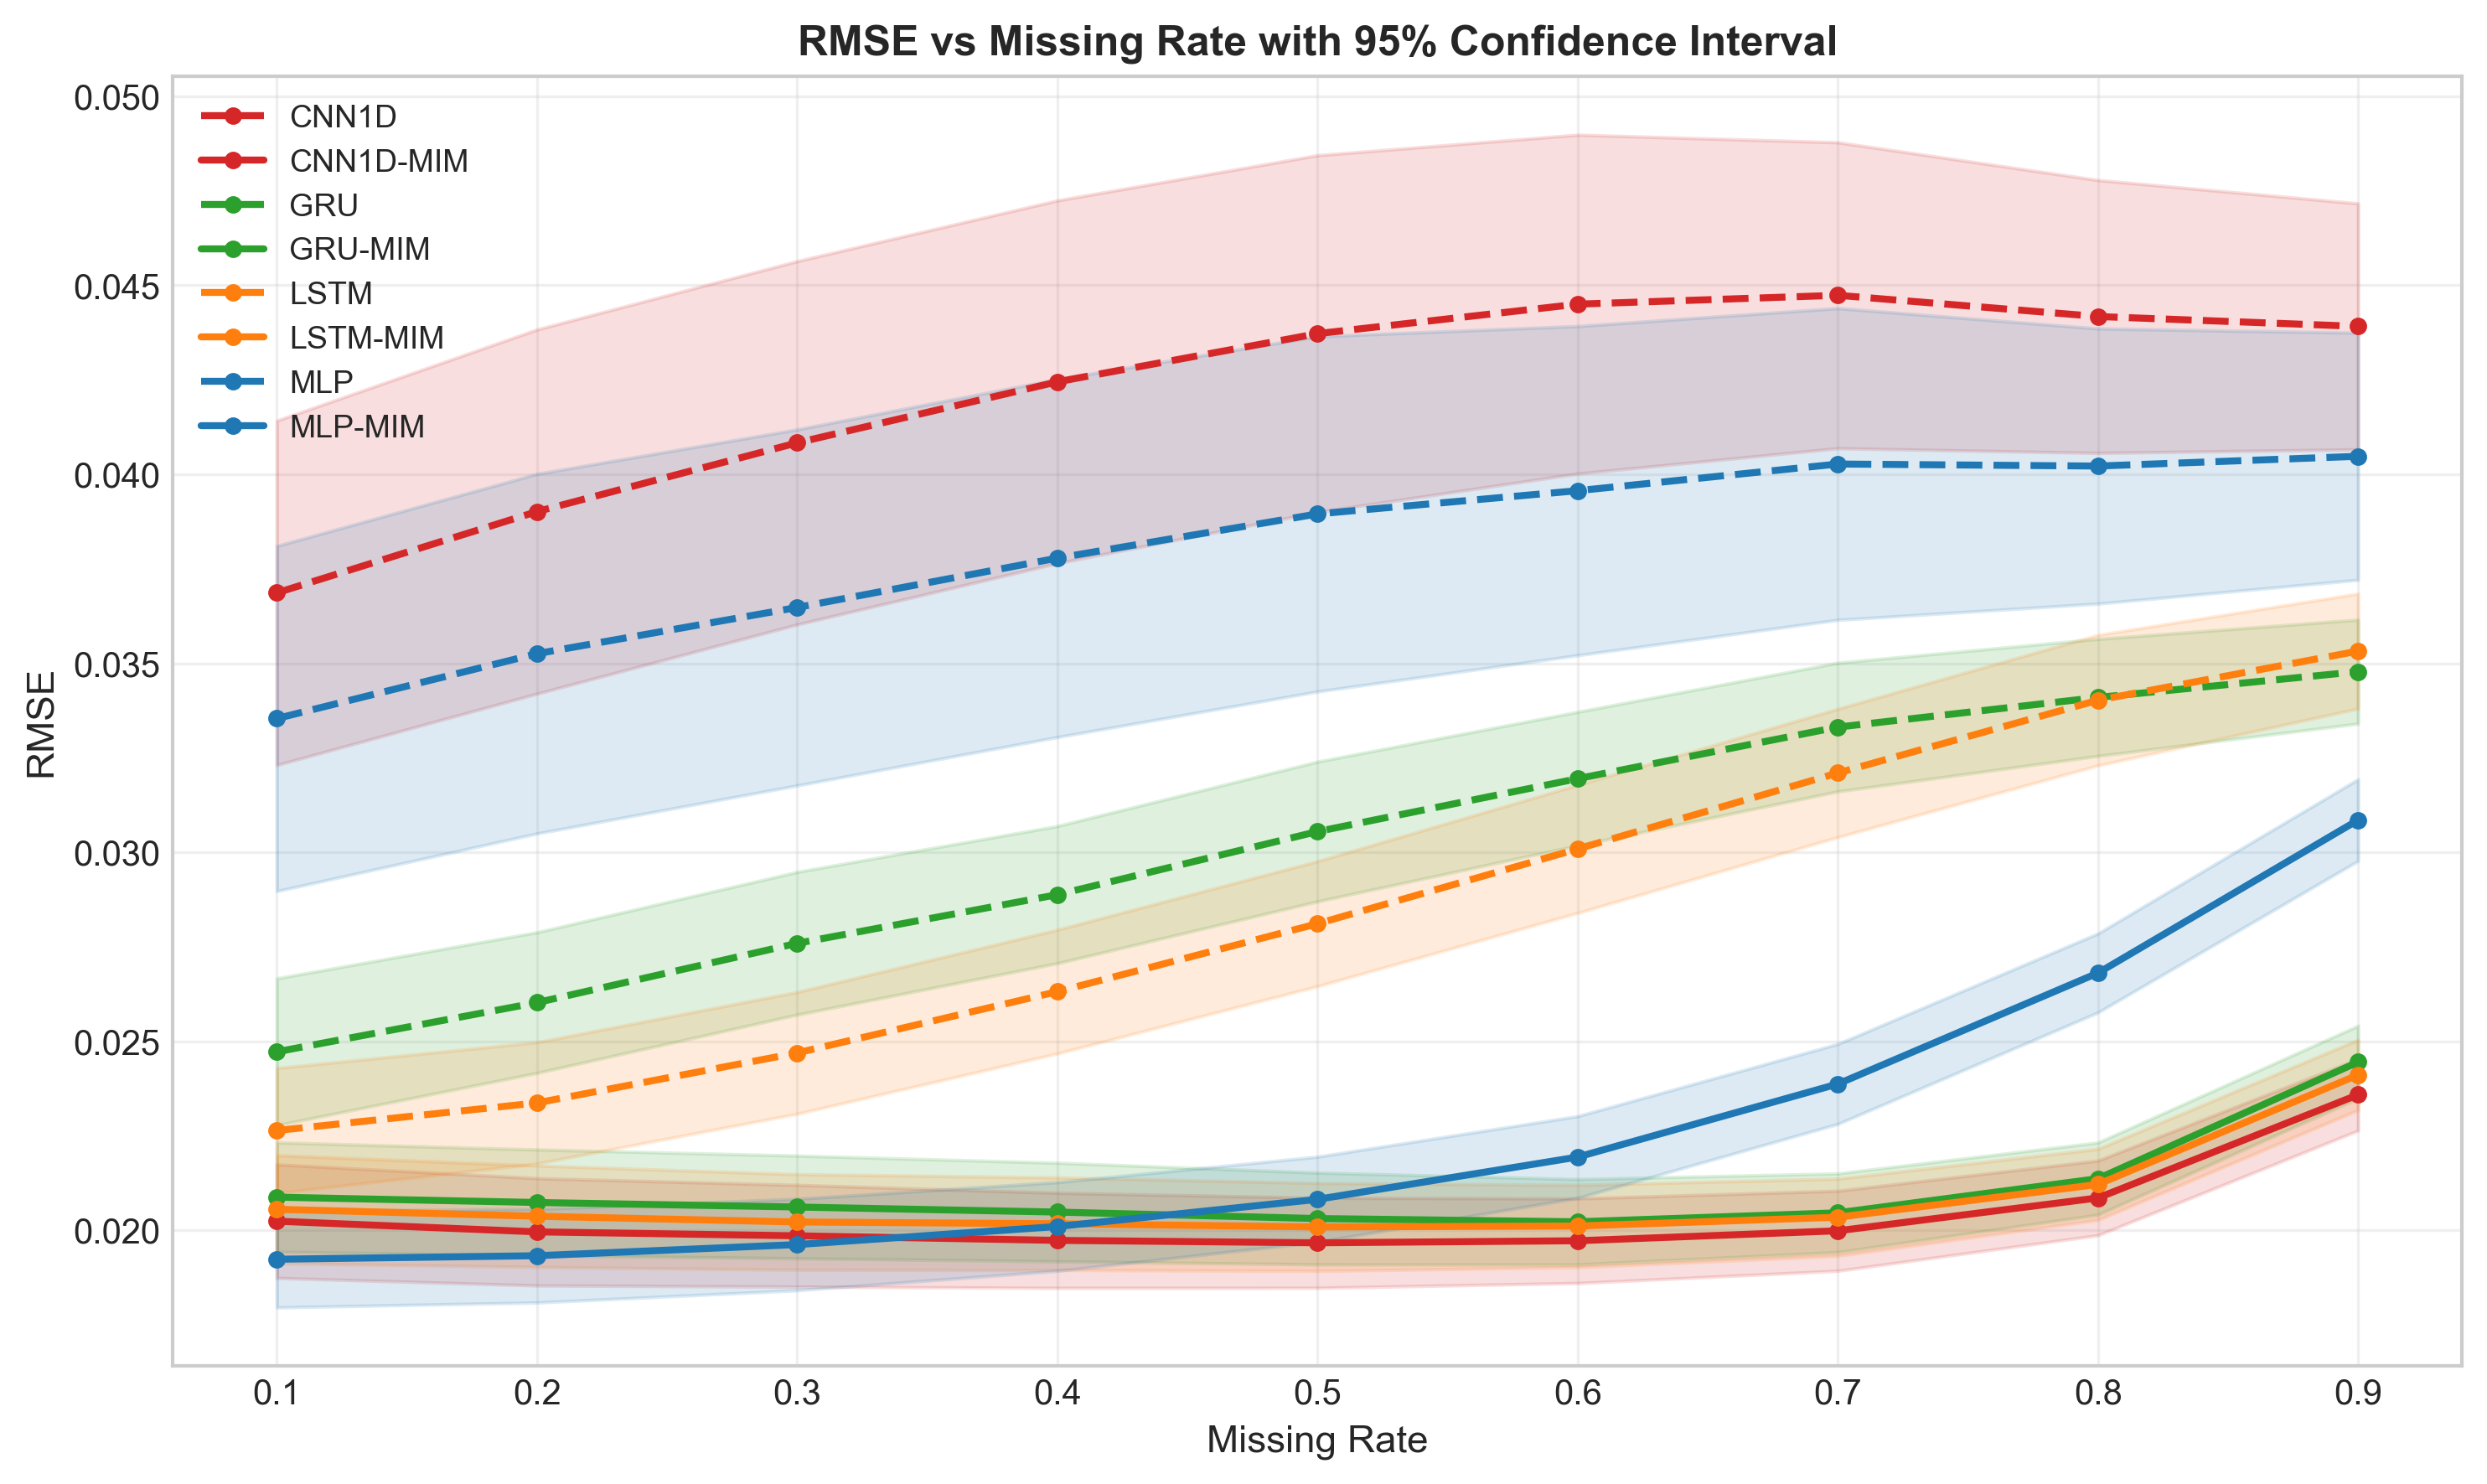
\includegraphics[width=\textwidth]{rmse_curves_ci.png}
        \caption{RMSE}
        \label{fig:rmse_all}
    \end{subfigure}
    \vskip 0.5em
    \begin{subfigure}[t]{0.58\textwidth}
        \centering
        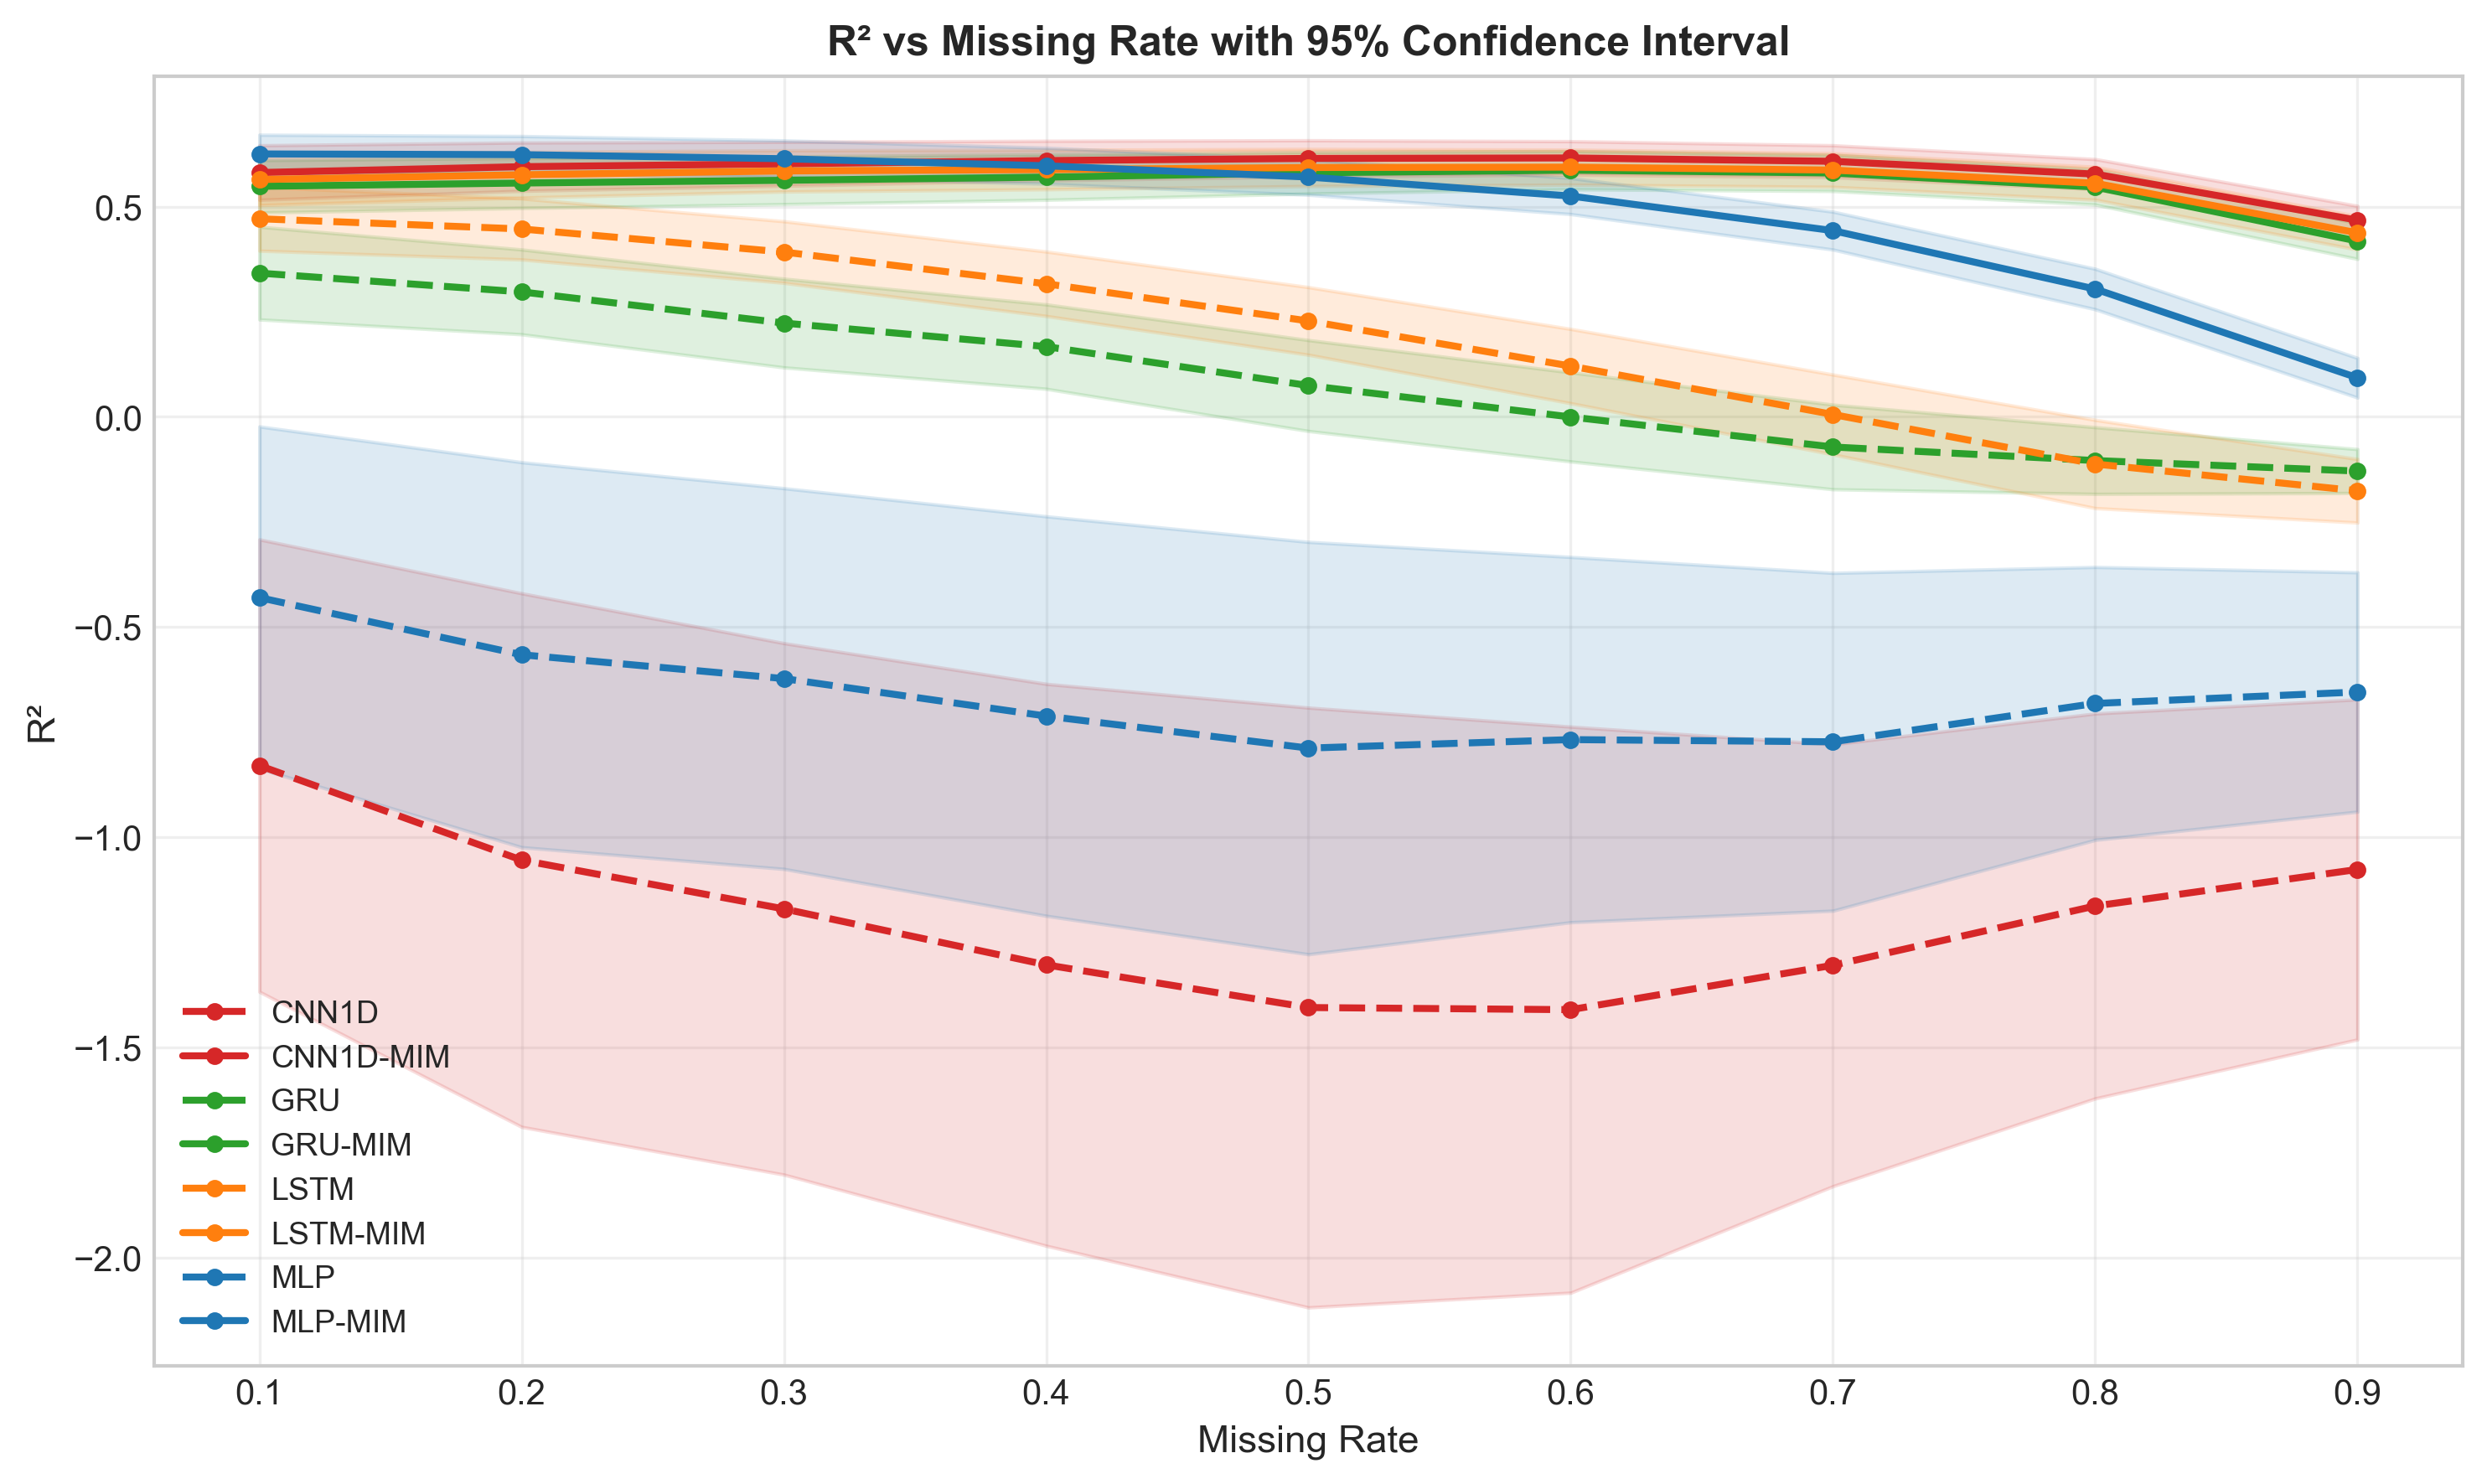
\includegraphics[width=\textwidth]{r2_curves_ci.png}
        \caption{R$^2$}
        \label{fig:r2_all}
    \end{subfigure}
    \caption{三种评价指标下的模型表现对比：(a) MAE；(b) RMSE；(c) R²。三种指标呈现一致的趋势，验证了MIM方法的有效性。}
    \label{fig:three_metrics}
\end{figure}

\end{document}
